\chapter{Results and Discussion}
\label{chap:results}

\section{Performance Evaluation Metrics}

To measure the performance of each model, the study used the same metrics used from previous works of CNN--TIC studies for both classification and financial evaluation \cite{maratkhan2021deep}. For classification performance, validation accuracy, test accuracy, and macro F1-score were used. These metrics are important to measure not only the total number of correct predictions, but also the balance of the model's performance in the Buy, Hold, and Sell classes.

For financial evaluation, final equity, mean annual return, and standard deviation of annual return were used. Final equity shows the total amount obtained after applying the trading strategy in the test period. The mean annual return measures the typical annual return of the strategy, while the standard deviation refers to the degree of variability of returns across years. In this way, the models are evaluated not only as classifiers but also as systems used in actual trading simulations.

\section{Implementation Details and Training Protocol}
All experiments in this study were performed on a workstation running Ubuntu 24.04.3 LTS. The system has an Intel Core i7-14700 processor, running at up to 5.4~GHz, 62~GB of system memory, and an NVIDIA GeForce RTX 4070 Ti GPU with 12~GB VRAM. 


All experiments in this chapter were conducted using the same preprocessing pipeline, labeling strategy, image construction procedure, and trading simulation rules presented in Chapter 3. The baseline model is CNN--TIC, which uses only technical indicators as input representation, while the proposed model CNN--MIC extends this representation by including macroeconomic indicators.

The two models were evaluated under five validation schemes, namely, Chronological Holdout Validation with Stratified K-Fold, Expanding-Window Walk-Forward Validation, Nested Walk-Forward Validation, Blocked Cross-Validation, and Blocked Cross-Validation with Partial Undersampling. Using multiple validation schemes is important to measure whether the performance of each model remains robust across different evaluation settings.

\section{Experimental Setups}
The experiments were organized into three major asset groups, blue-chip stocks, penny stocks, and cryptocurrency. For blue-chip stocks, Ayala Corporation (AC), Jollibee Foods Corporation (JFC), and SM Investments Corporation (SMI) were examined. For penny stocks, these included PH Resorts Group (PHR), United Paragon Mining Corporation (UPM), and Araneta Properties (ARA). Lastly for cryptocurrency, Bitcoin (BTC), Litecoin (LTC), and XRP were examined.

\subsection{Experiment 1: Comparing CNN--TIC and CNN--MIC with Different Validation Schemes}

The first experiment was conducted to examine how the performance of CNN--TIC and CNN--MIC differed across the five validation schemes used in the study. This experiment examined how the inclusion of macroeconomic indicators affected validation performance across different evaluation setups.

\subsection{Experiment 2: Benchmarking Test Classification and Financial Performance}

The second experiment was conducted to compare the performance of two models on out-of-sample data using accuracy, Macro F1-score, and financial metrics such as annualized return. This experiment aimed to determine how the inclusion of macroeconomic indicators affected both predictive performance and trading performance.

\subsection{Experiment 3: SHAP-Based Interpretation of CNN--MIC Across Validation Schemes}

The third experiment was conducted to interpret the behavior of CNN--MIC using SHAP analysis. The main discussion focuses on Ayala Corporation (AC) across the validation schemes, while additional predicted-class SHAP row importance plots for selected assets under BCV-PU are presented in Appendix A.4. Unlike the first two experiments, which compared the numerical performance of CNN--TIC and CNN--MIC across multiple assets and asset groups, this experiment focused on one representative stock in order to examine how feature contribution changes under different validation schemes. The analysis aimed to determine whether the model remained primarily driven by technical indicators across all evaluation settings and to identify which macroeconomic variables provided supporting information in each scheme.


\section{Results and Discussion}
The results in this chapter are organized according to the three experiments presented in the previous section. For the presentation of tables, the validation schemes are abbreviated as CHV-SKF for Chronological Holdout Validation with Stratified K-Fold, EW-WFV for Expanding-Window Walk-Forward Validation, NWFV for Nested Walk-Forward Validation, BCV for Blocked Cross-Validation, and BCV-PU for Blocked Cross-Validation with Partial Undersampling.

\subsection{Experiment 1: Comparison of Validation Performance Across Validation Schemes}

Table~\ref{tab:val_bluechip} to Table~\ref{tab:val_crypto} in Appendix~\ref{app:experiment1_tables} show the validation performance of CNN--TIC and CNN--MIC on the three asset groups. The numerical results show that the effect of adding macroeconomic indicators is not uniform across all assets and validation schemes. Instead, the observed gains vary depending on both the characteristics of the asset and the structure of the validation procedure. This suggests that the contribution of macroeconomic information is conditional rather than universal. To better compare the validation behavior of the two models, the validation accuracy scores were summarized using box plots for each asset.


\begin{center}
	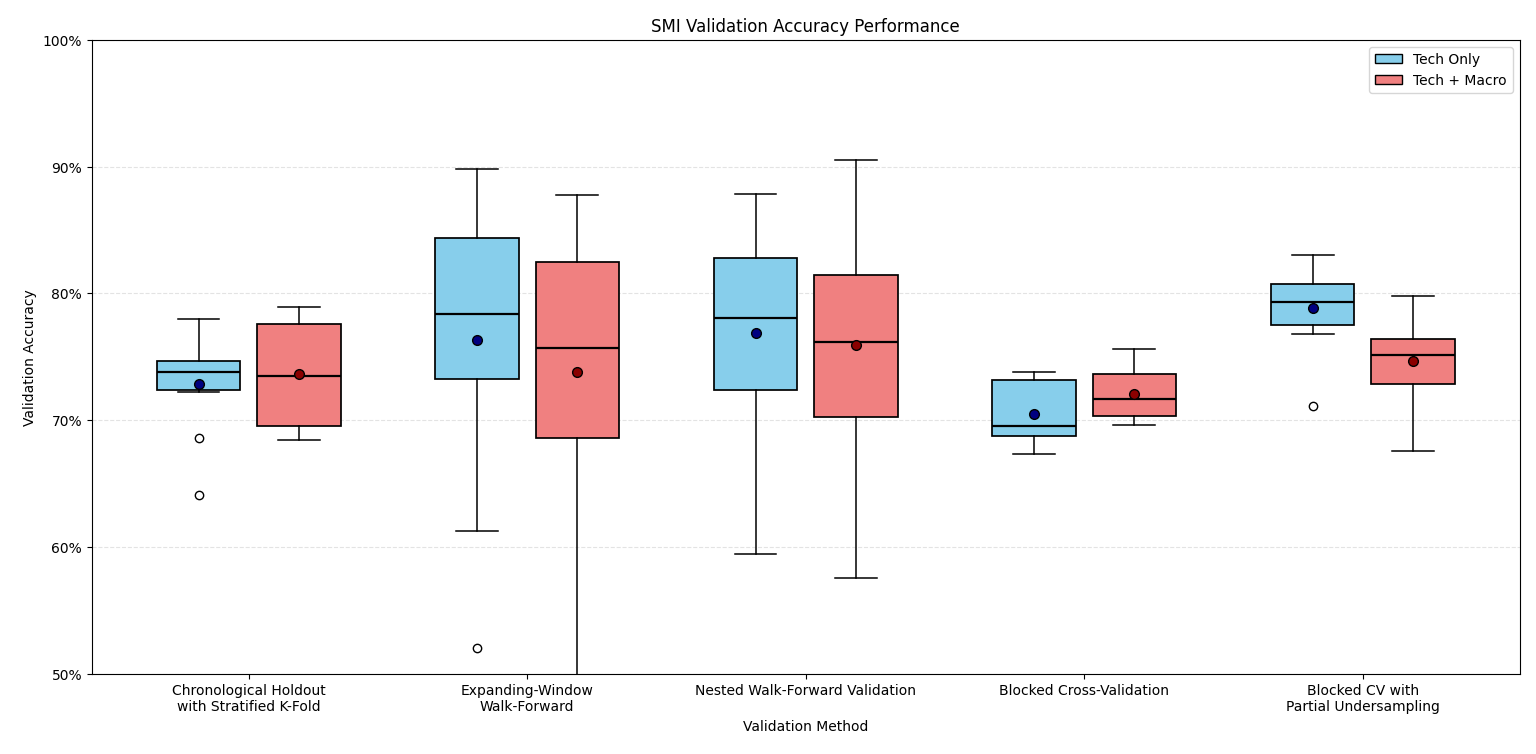
\includegraphics[width=0.8\textwidth]{../figures/SMI_Val.png}\\
	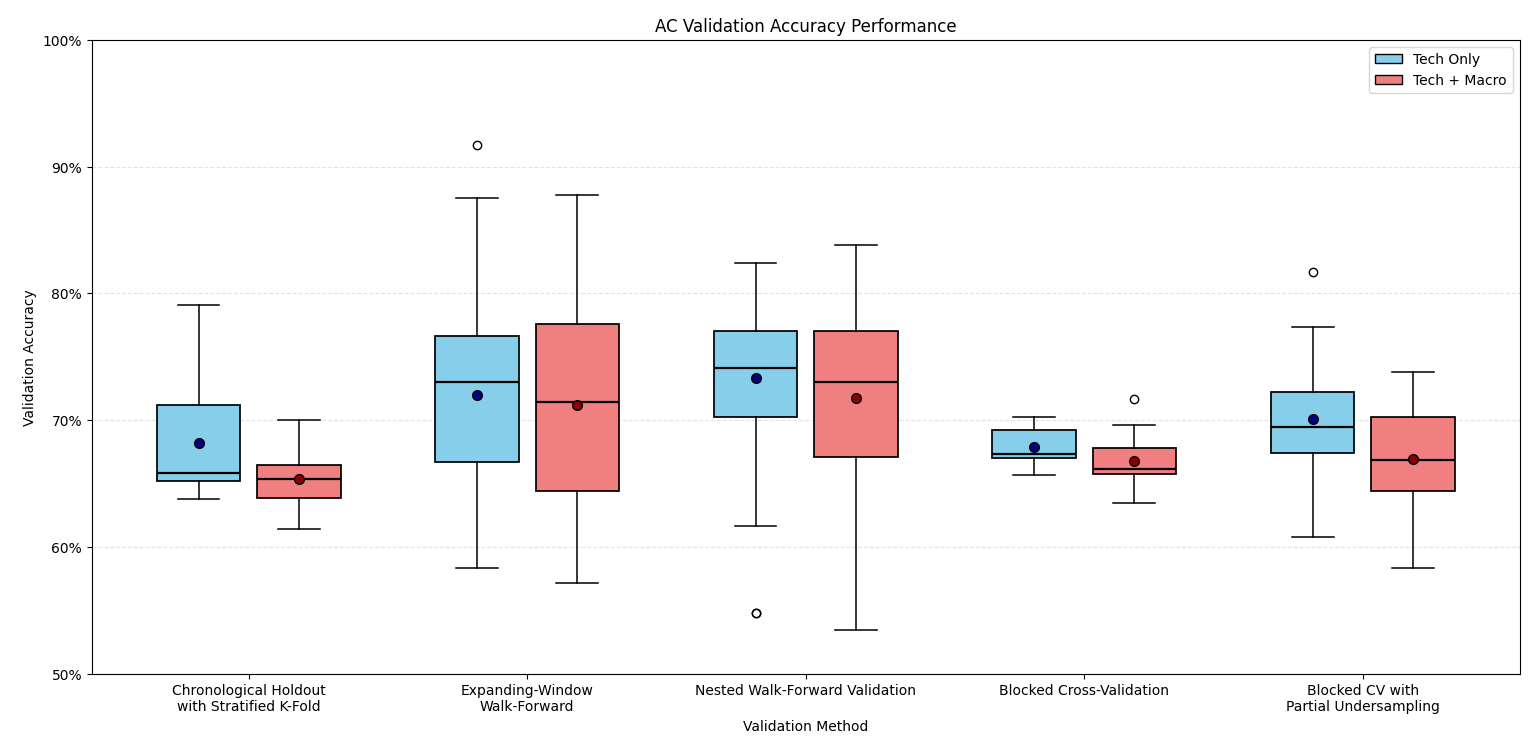
\includegraphics[width=0.8\textwidth]{../figures/AC_Val.png}\\
	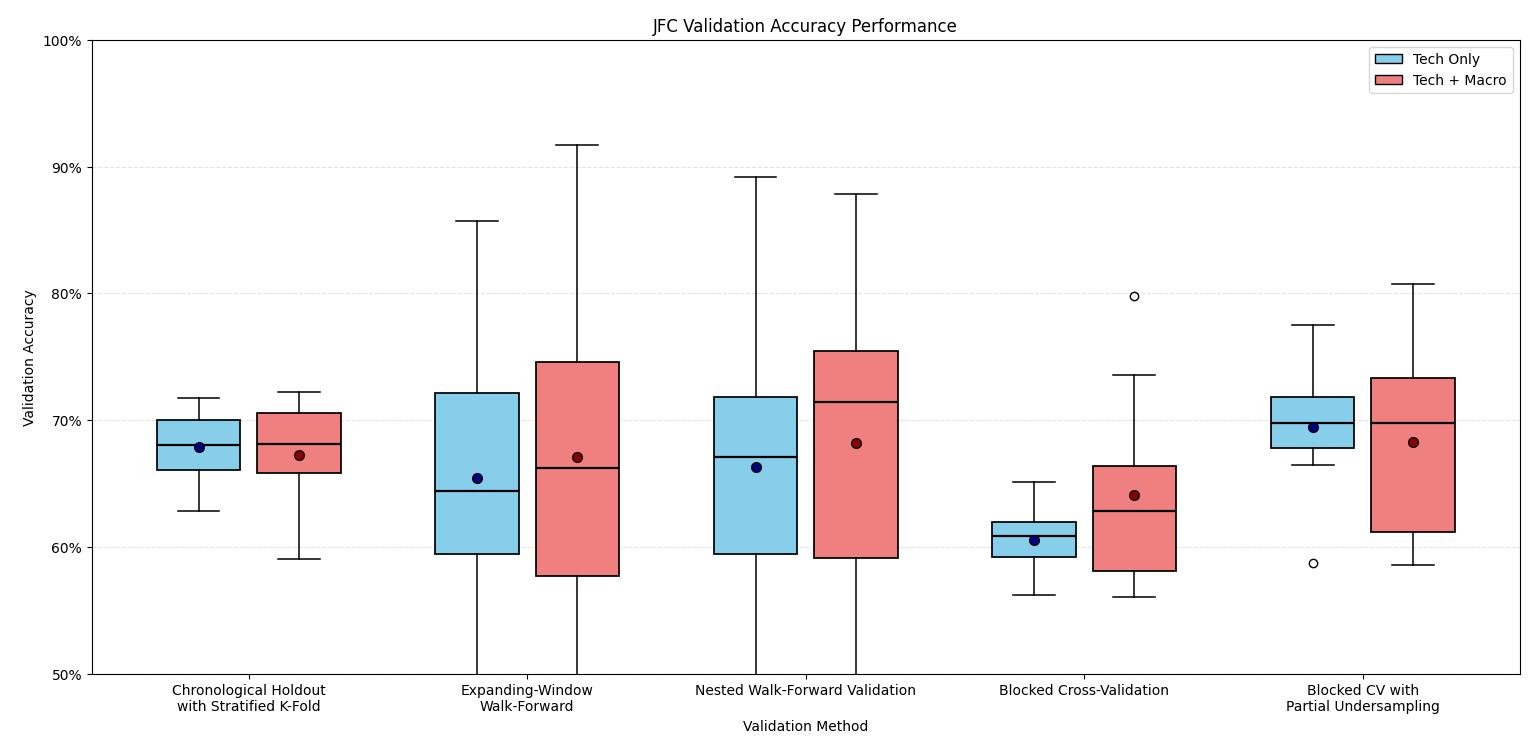
\includegraphics[width=0.8\textwidth]{../figures/JFC_Val.png}
	
	\captionof{figure}{Validation accuracy performance of CNN--TIC and CNN--MIC across selected blue-chip stocks}
	\label{fig:val_bluechip_boxplots}
\end{center}

Figure~\ref{fig:val_bluechip_boxplots} shows the validation accuracy performance of CNN--TIC and CNN--MIC across SMI, AC, and JFC. For the blue-chip group, the results were mixed. CNN--MIC was more competitive in selected settings for AC and JFC, particularly in Expanding-Window Walk-Forward and some Blocked Cross-Validation-based schemes. However, CNN--TIC remained stronger in several Nested Walk-Forward Validation and Blocked Cross-Validation with Partial Undersampling results, especially for SMI. This indicates that macroeconomic integration does not consistently improve validation performance for large-cap assets.

\begin{center}
	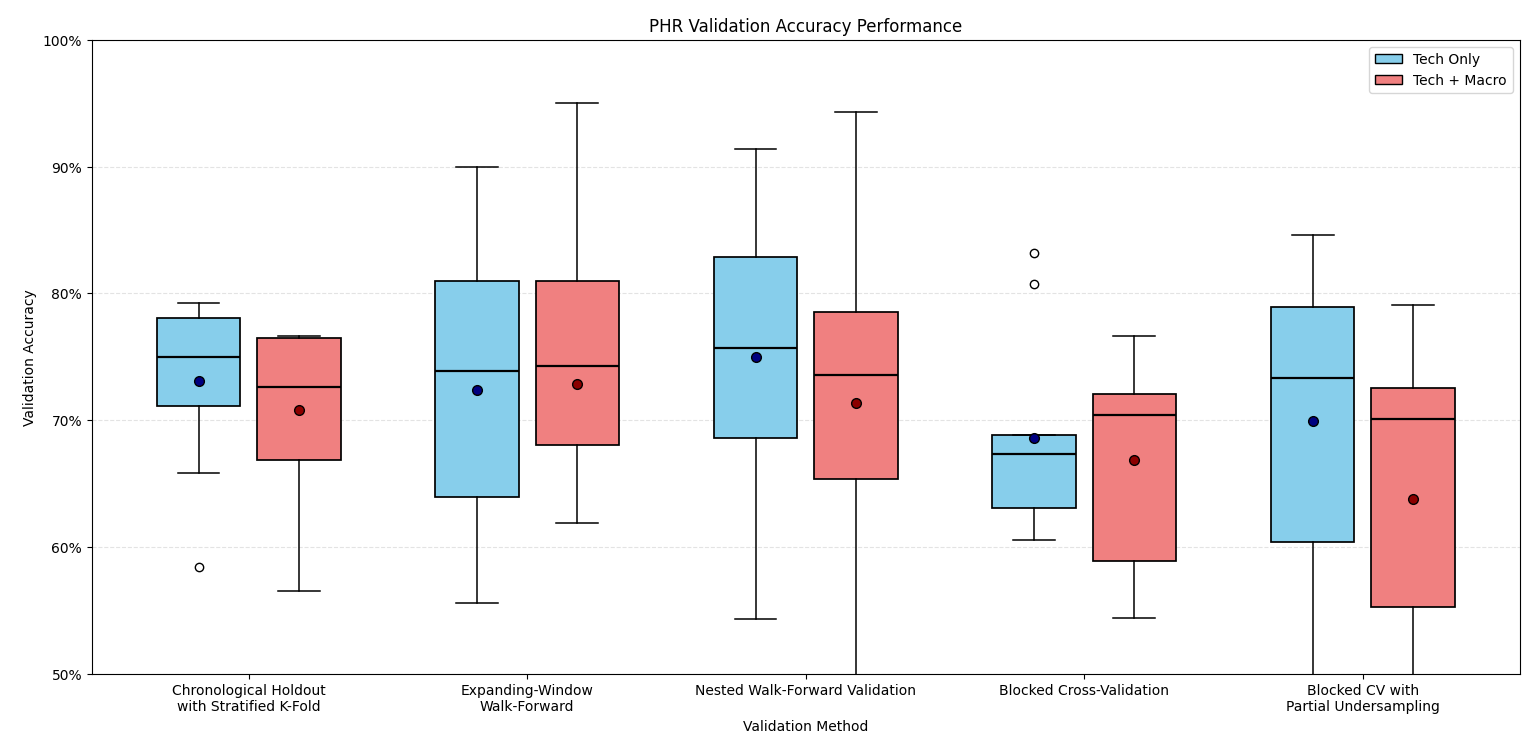
\includegraphics[width=0.8\textwidth]{../figures/PHR_Val.png}
	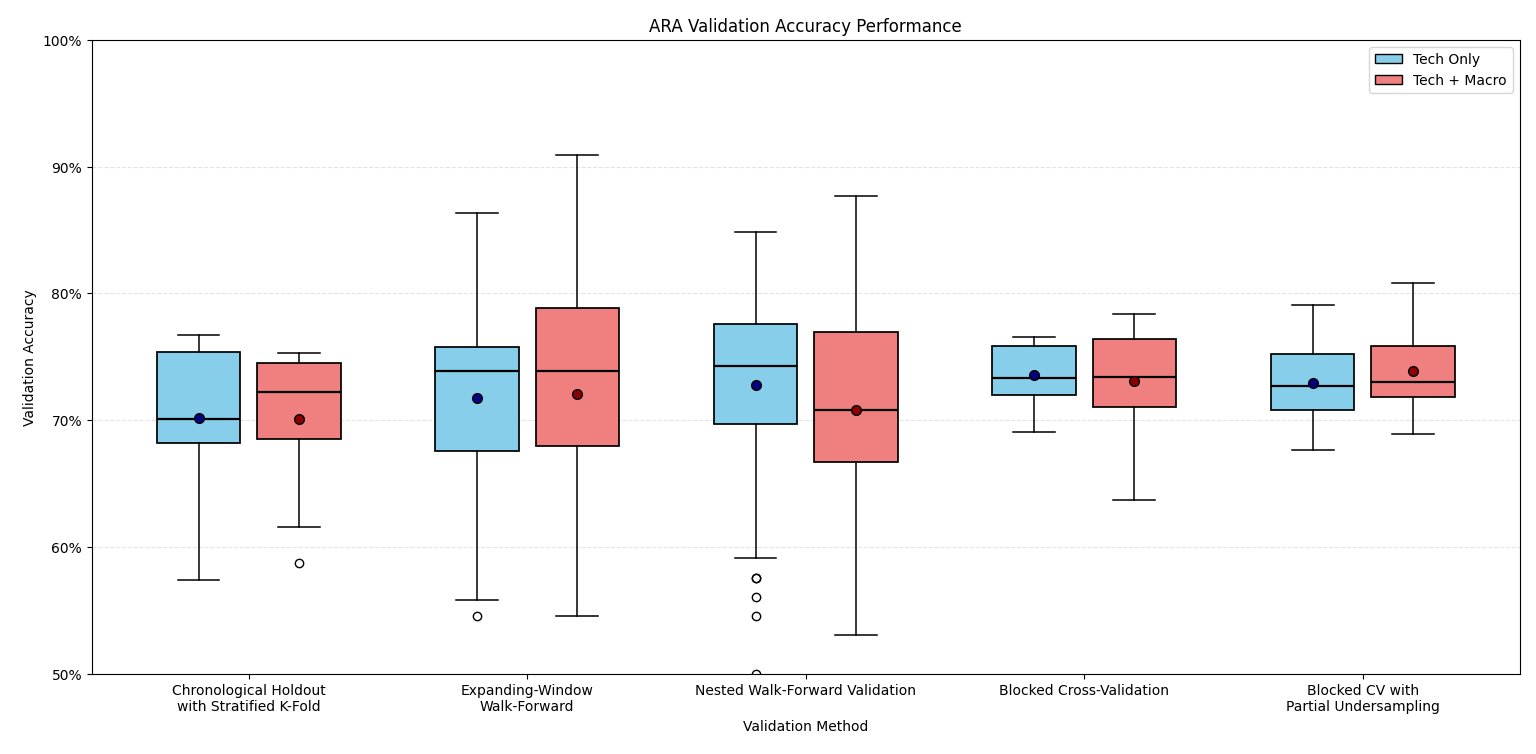
\includegraphics[width=0.8\textwidth]{../figures/ARA_Val.png}
	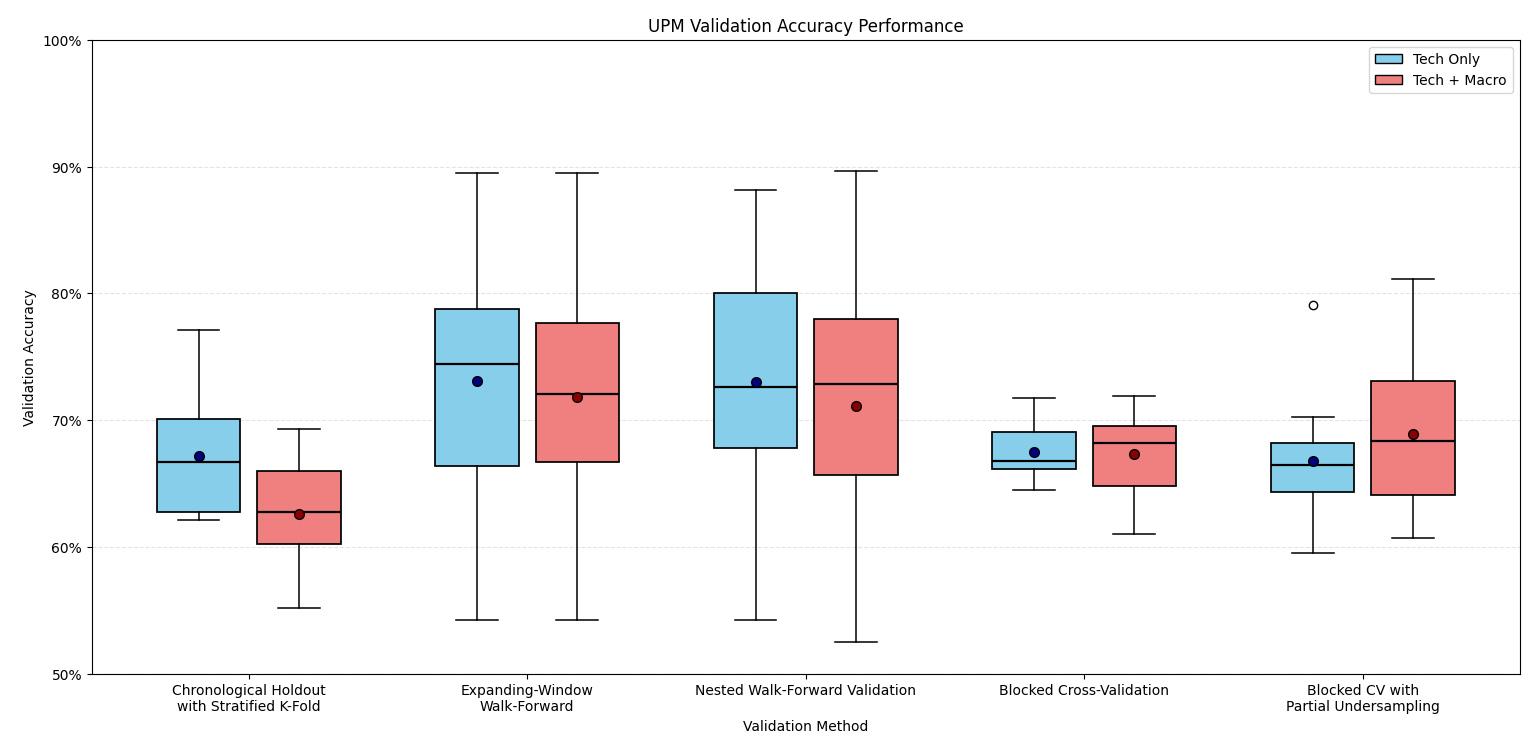
\includegraphics[width=0.8\textwidth]{../figures/UPM_Val.png}
	
	\captionof{figure}{Validation accuracy performance of CNN--TIC and CNN--MIC across selected penny stocks}
	\label{fig:val_penny_boxplots}
\end{center}

Figure~\ref{fig:val_penny_boxplots} shows the validation accuracy performance of CNN--TIC and CNN--MIC across PHR, ARA, and UPM. For penny stocks, CNN--TIC remained more competitive in UPM and PHR across most schemes. In contrast, CNN--MIC showed its clearest advantage in ARA, particularly in selected validation settings. These results suggest that the effect of macroeconomic indicators in low-priced equities is also selective rather than uniform.

\begin{center}
	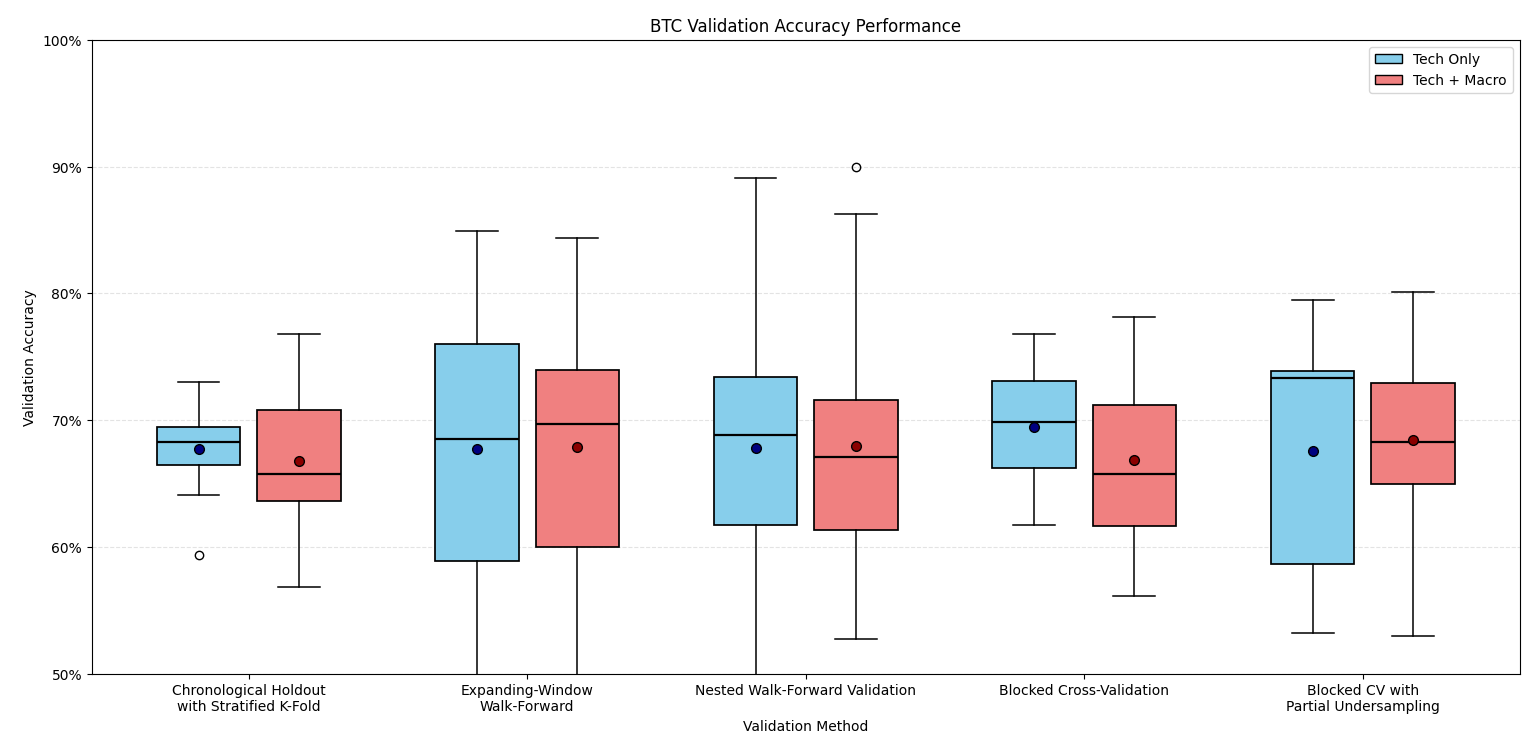
\includegraphics[width=0.8\textwidth]{../figures/BTC_Val.png}
	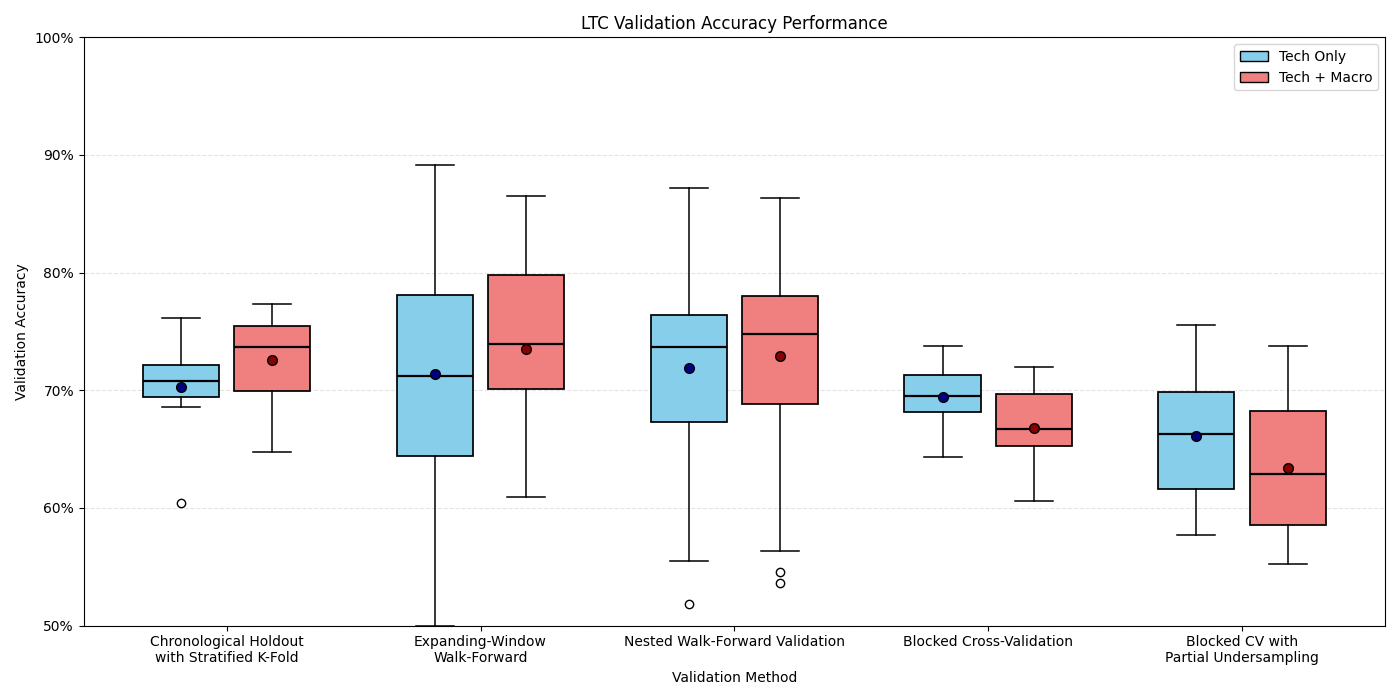
\includegraphics[width=0.8\textwidth]{../figures/LTC_Val.png}
	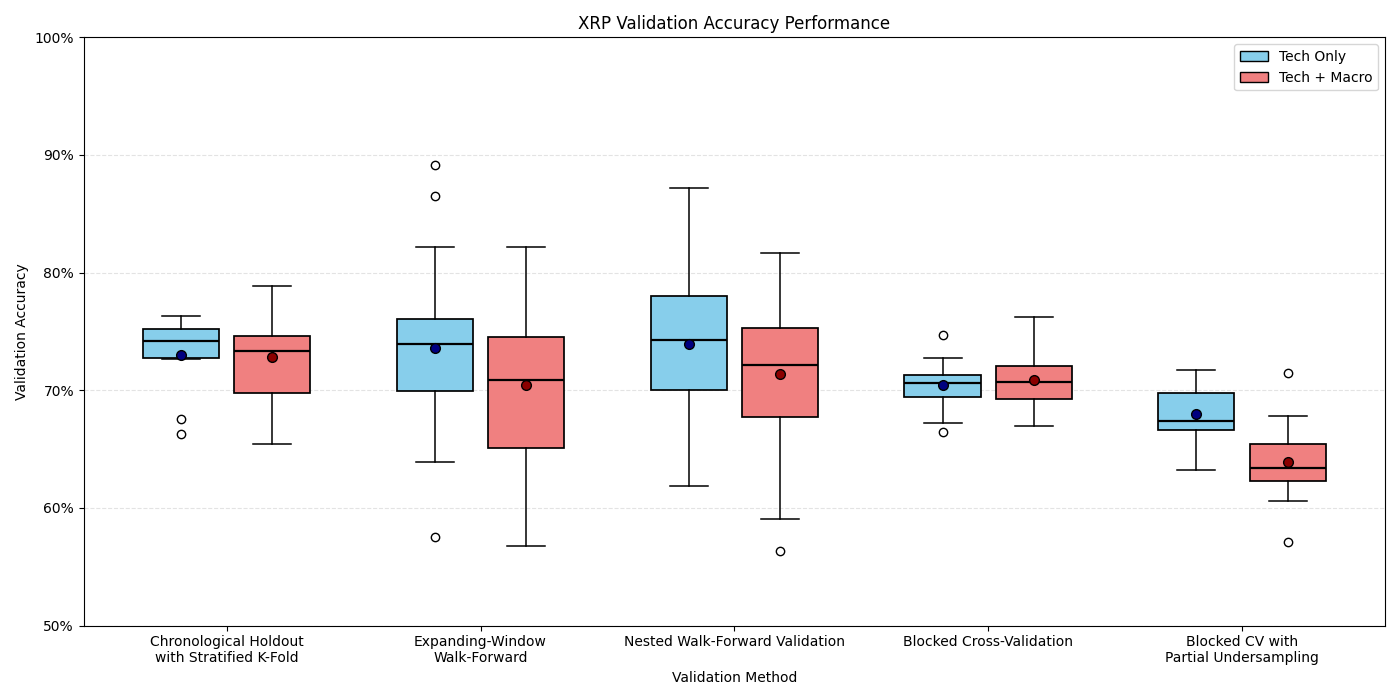
\includegraphics[width=0.8\textwidth]{../figures/XRP_Val.png}
	
	\captionof{figure}{Validation accuracy performance of CNN--TIC and CNN--MIC across selected cryptocurrency assets}
	\label{fig:val_crypto_boxplots}
\end{center}

Figure~\ref{fig:val_crypto_boxplots} shows the validation accuracy performance of CNN--TIC and CNN--MIC across BTC, LTC, and XRP. For cryptocurrencies, CNN--MIC showed clearer gains in BTC and LTC under selected validation schemes, particularly in Expanding-Window Walk-Forward and Nested Walk-Forward Validation. However, CNN--TIC remained stronger for XRP across most settings. Among the three asset groups, the cryptocurrency group shows the most visible but still asset-specific benefit from macroeconomic integration.



\subsection{Experiment 2: Comparison of Test Classification and Financial Performance}
This experiment compares CNN--TIC and CNN--MIC not only as classifiers, but also as Buy, Hold, and Sell trading systems. In the financial evaluation, each predicted class is treated as a trading signal and executed using the same backtesting rules described in Algorithm~\ref{alg:financial-evaluation}. The comparison therefore measures whether the Buy, Hold, and Sell decisions produced by the technical-only model or the macroeconomic-integrated model lead to stronger portfolio outcomes.

It is important to distinguish classification performance from financial performance. Accuracy measures how often the predicted class matches the ground-truth label. However, profitability depends on the timing, direction, and economic consequence of each predicted action. A model may obtain higher accuracy by correctly predicting many Hold instances, but still miss fewer Buy or Sell signals that have larger effects on portfolio value. 
Similarly, a model with lower accuracy may still generate better financial results if its correct predictions occur near more profitable entry and exit points. This distinction is important in trading systems because economic value is affected not only by predictive correctness, but also by transaction costs, class imbalance, return magnitude, and the sequence of executed trades \cite{moosa2015directional,fischer2021feature,ozbayoglu2020deep}. Therefore, this study evaluates the models using both classification metrics and trading metrics.

Tables~\ref{tab:test_bluechip} to~\ref{tab:fin_crypto} in Appendix~\ref{app:experiment2_tables} present the complete out-of-sample classification and financial performance values of CNN--TIC and CNN--MIC. 
The classification results show how well the models predicted the Buy, Hold, and Sell labels on unseen data. The financial results show whether these predicted actions translated into higher final equity under the fixed trading simulation. This distinction is necessary because a higher test accuracy does not automatically imply a more profitable strategy. 

In trading, the value of a prediction depends on when the signal occurs and how much price movement follows after the executed action \cite{moosa2015directional,fischer2021feature}. To make the comparison clearer, the test accuracy and final equity results were summarized using grouped bar charts for each asset group.

The financial comparison is based on the Buy, Hold, and Sell predictions generated by each model. CNN--TIC produces these actions from the technical-only image representation, while CNN--MIC produces the same action classes from the combined technical and macroeconomic image representation. Both models are evaluated with identical starting capital, commission, take-profit, and stop-loss rules.

\begin{center}
	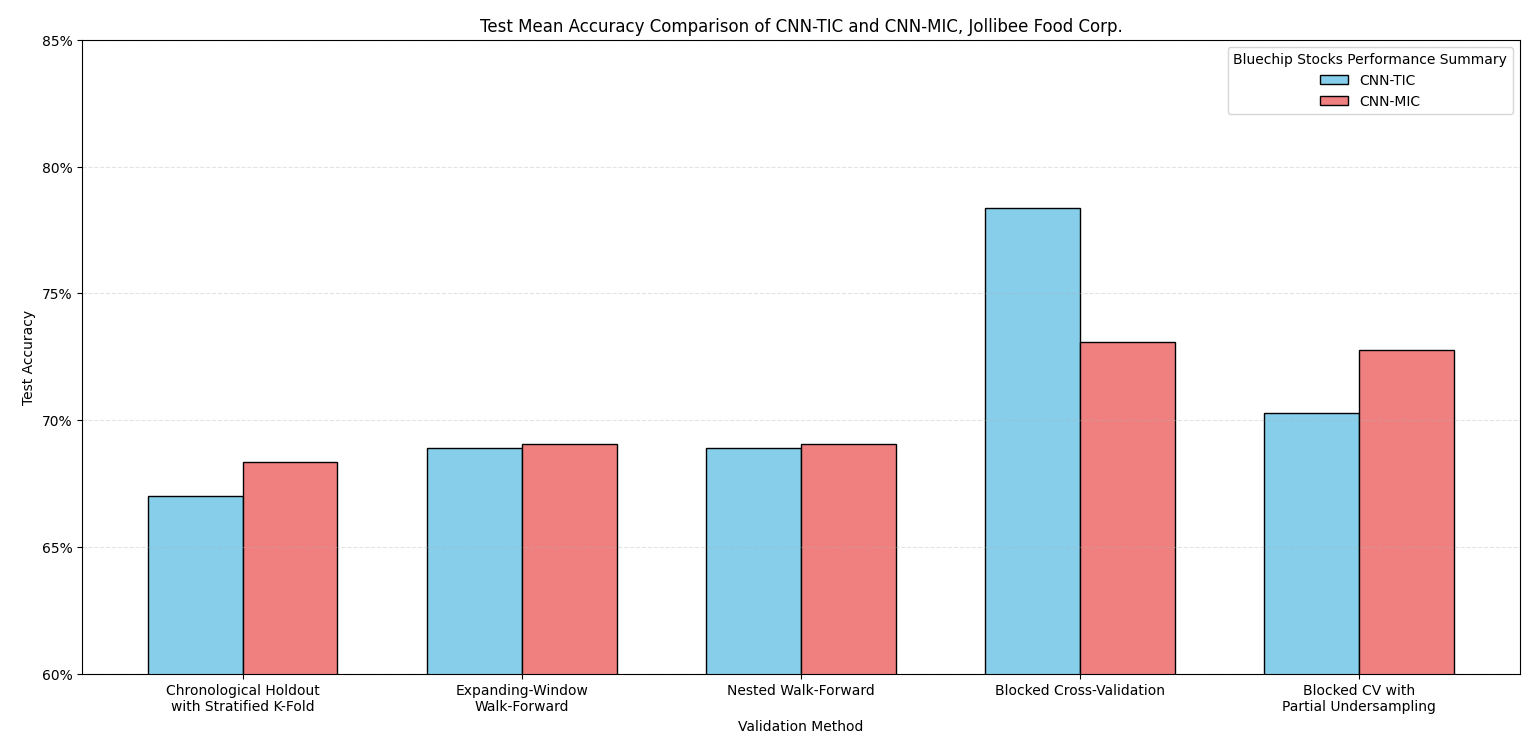
\includegraphics[width=0.8\textwidth]{../figures/JFC_TestAccuracy.png}
	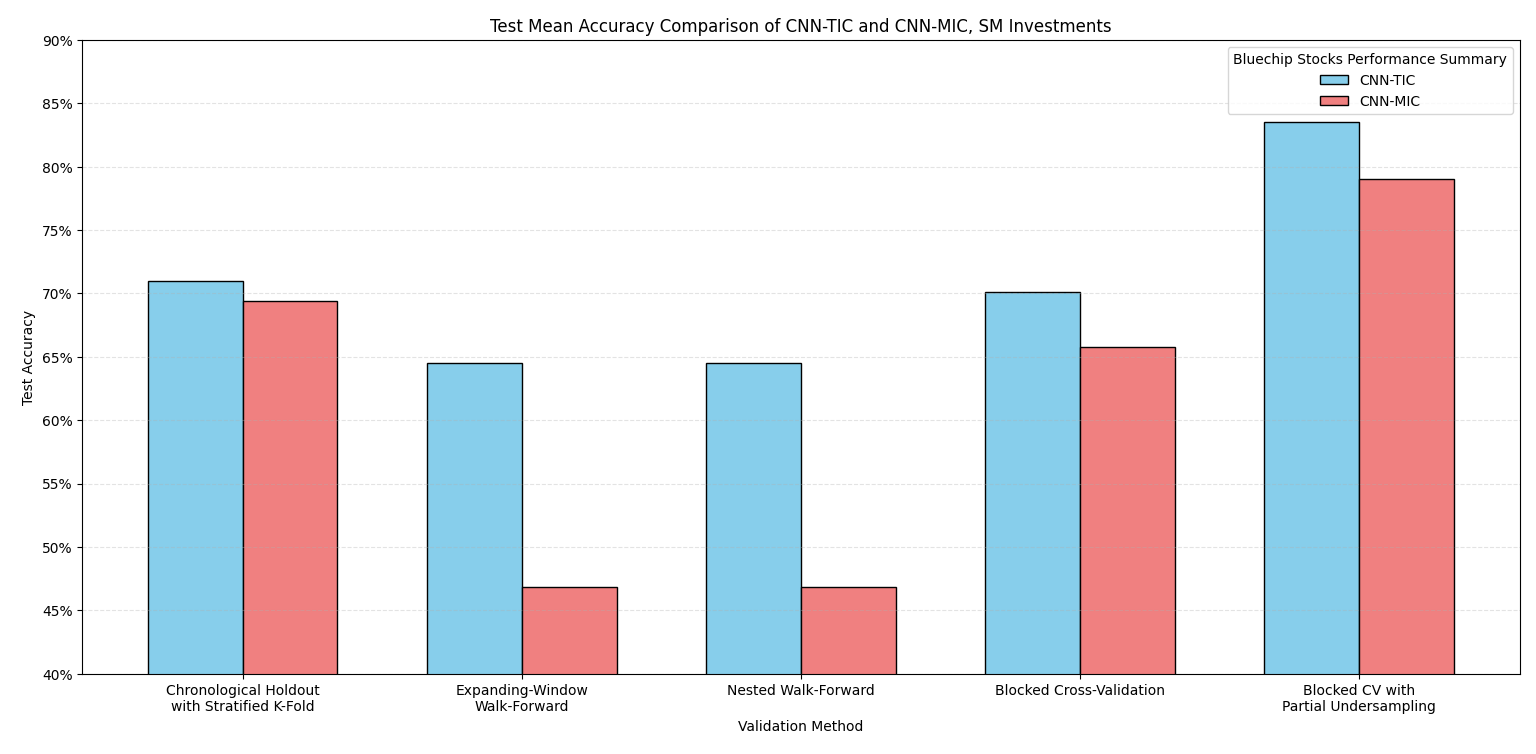
\includegraphics[width=0.8\textwidth]{../figures/SMI_TestAccuracy.png}
	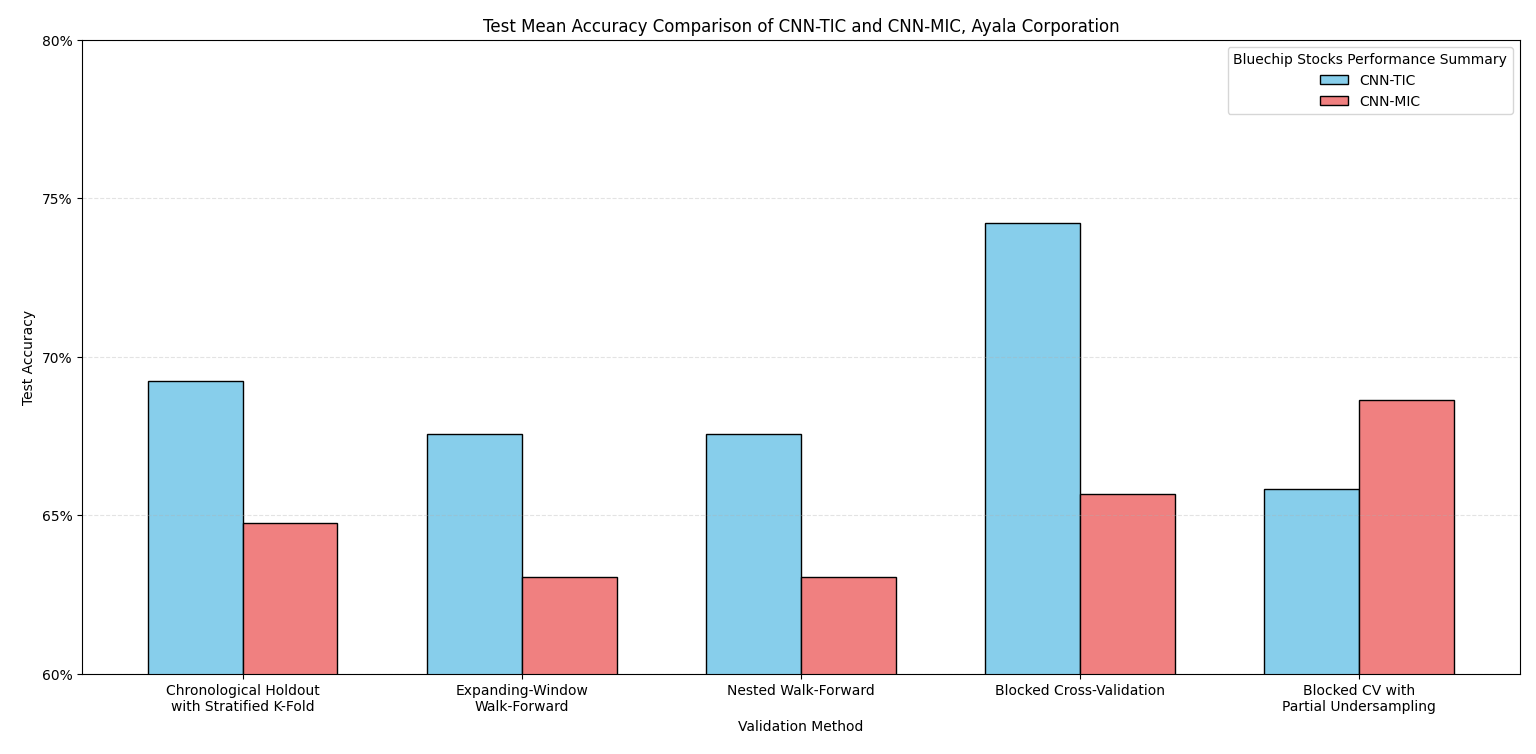
\includegraphics[width=0.8\textwidth]{../figures/AC_TestAccuracy.png}
	
	\captionof{figure}{Test accuracy performance of CNN--TIC and CNN--MIC across selected blue-chip stocks}
	\label{fig:test_bluechip_barplots}
\end{center}

\begin{center}
	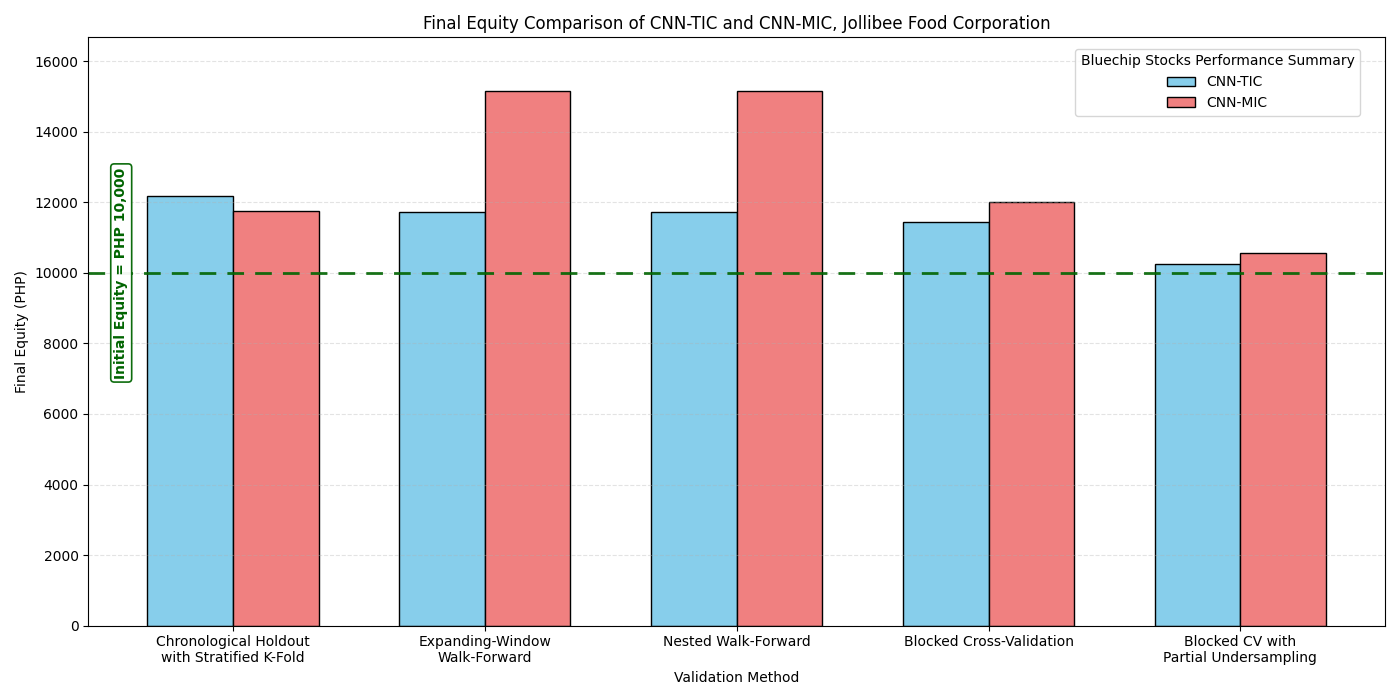
\includegraphics[width=0.8\textwidth]{../figures/JFC_FinancialAccuracy.png}
	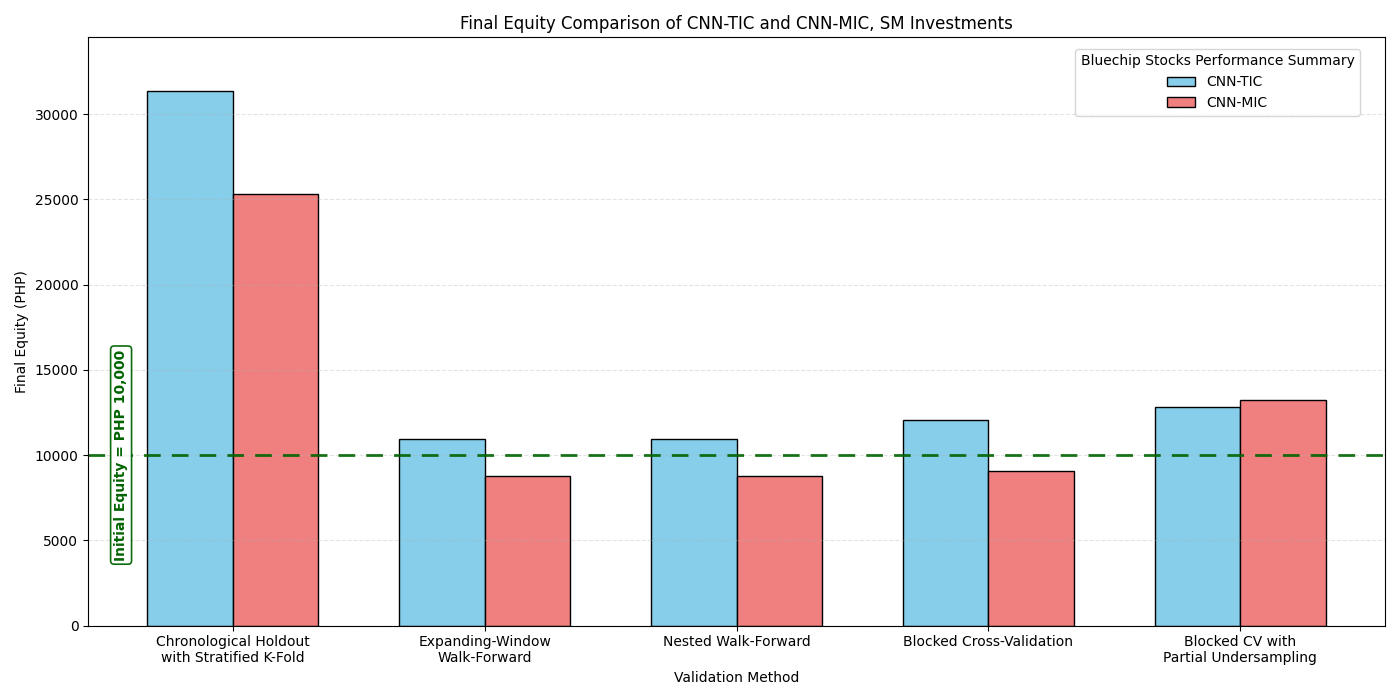
\includegraphics[width=0.8\textwidth]{../figures/SMI_FinancialAccuracy.png}
	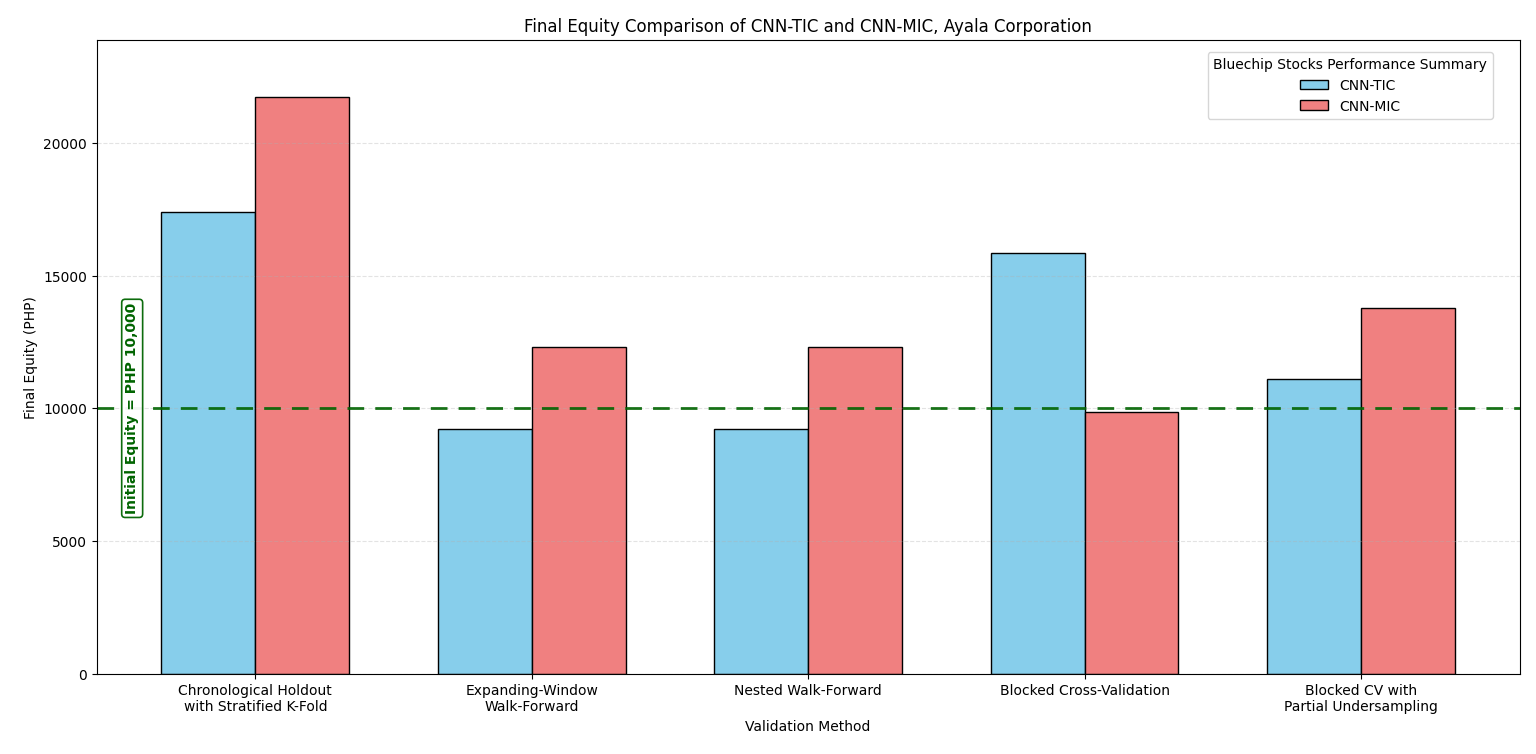
\includegraphics[width=0.8\textwidth]{../figures/AC_FinancialAccuracy.png}
	
	\captionof{figure}{Final equity performance of CNN--TIC and CNN--MIC across selected blue-chip stocks}
	\label{fig:fin_bluechip_barplots}
\end{center}

Figures~\ref{fig:test_bluechip_barplots} and~\ref{fig:fin_bluechip_barplots} show the test accuracy and final equity performance of CNN--TIC and CNN--MIC across the selected blue-chip stocks. Across this group, the out-of-sample classification results remained mixed. CNN--MIC was more competitive for JFC and selected AC settings, while CNN--TIC remained stronger for SMI and several BCV-based results. The financial results followed a similar asset-specific pattern. CNN--MIC produced stronger final equity for AC and selected JFC settings, whereas CNN--TIC remained stronger for SMI in most configurations. This suggests that macroeconomic information can help in selected large-cap cases, but the gains do not transfer consistently across all blue-chip assets.

\begin{center}
	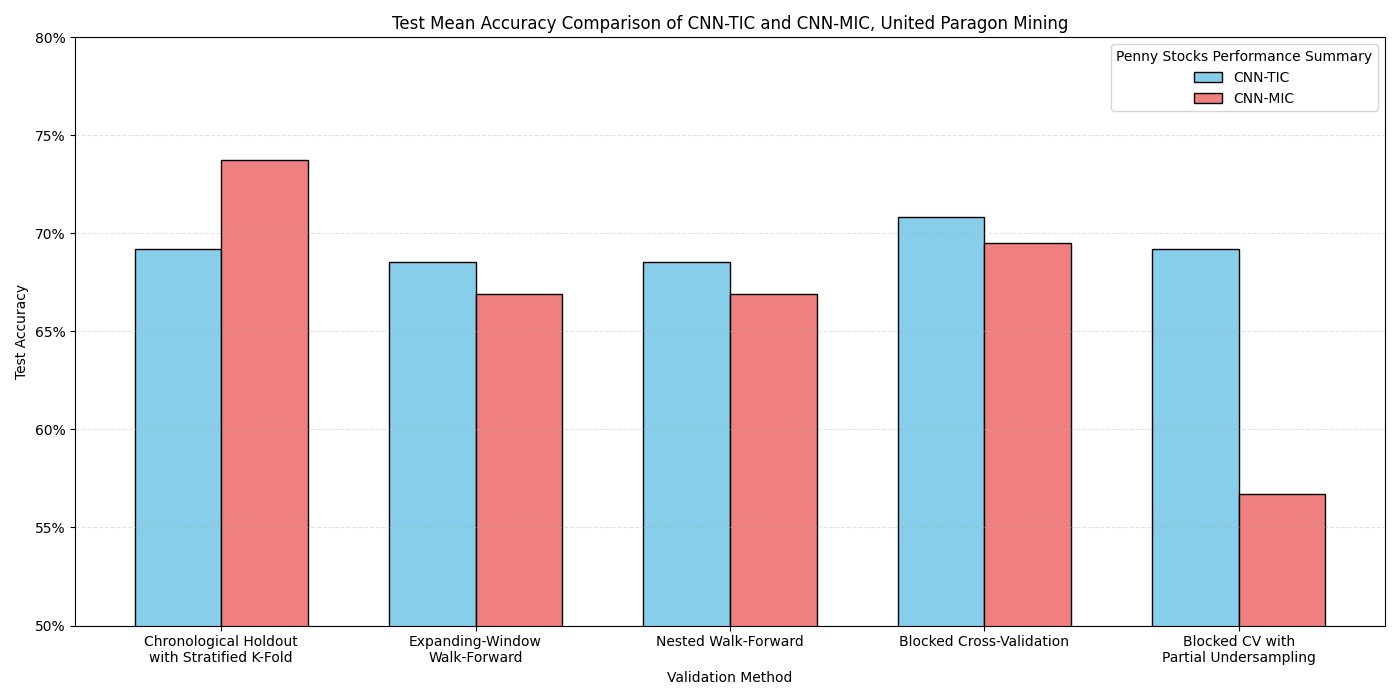
\includegraphics[width=0.8\textwidth]{../figures/UPM_TestAccuracy.png}
	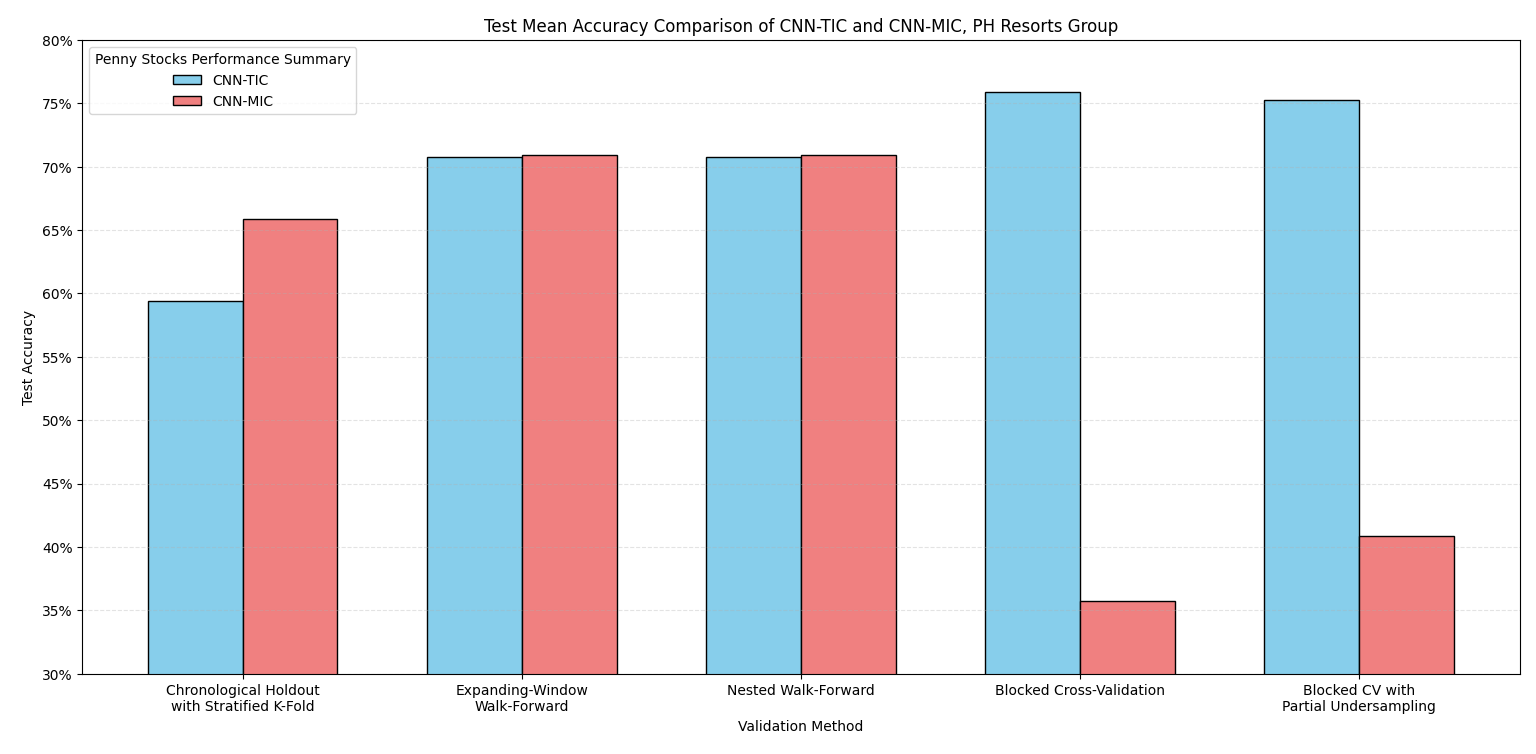
\includegraphics[width=0.8\textwidth]{../figures/PHR_TestAccuracy.png}
	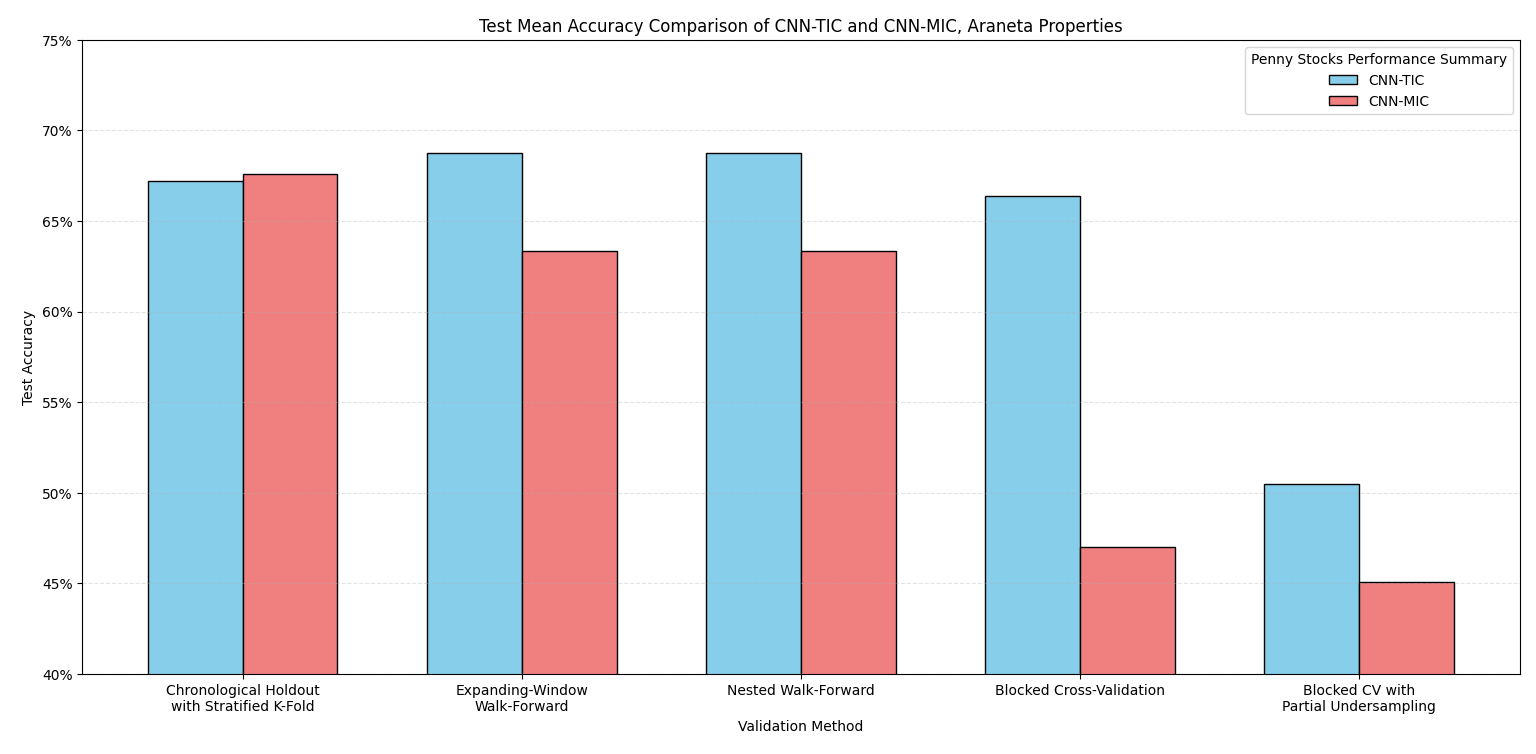
\includegraphics[width=0.8\textwidth]{../figures/ARA_TestAccuracy.png}
	
	\captionof{figure}{Test accuracy performance of CNN--TIC and CNN--MIC across selected penny stocks}
	\label{fig:test_penny_barplots}
\end{center}

\begin{center}
	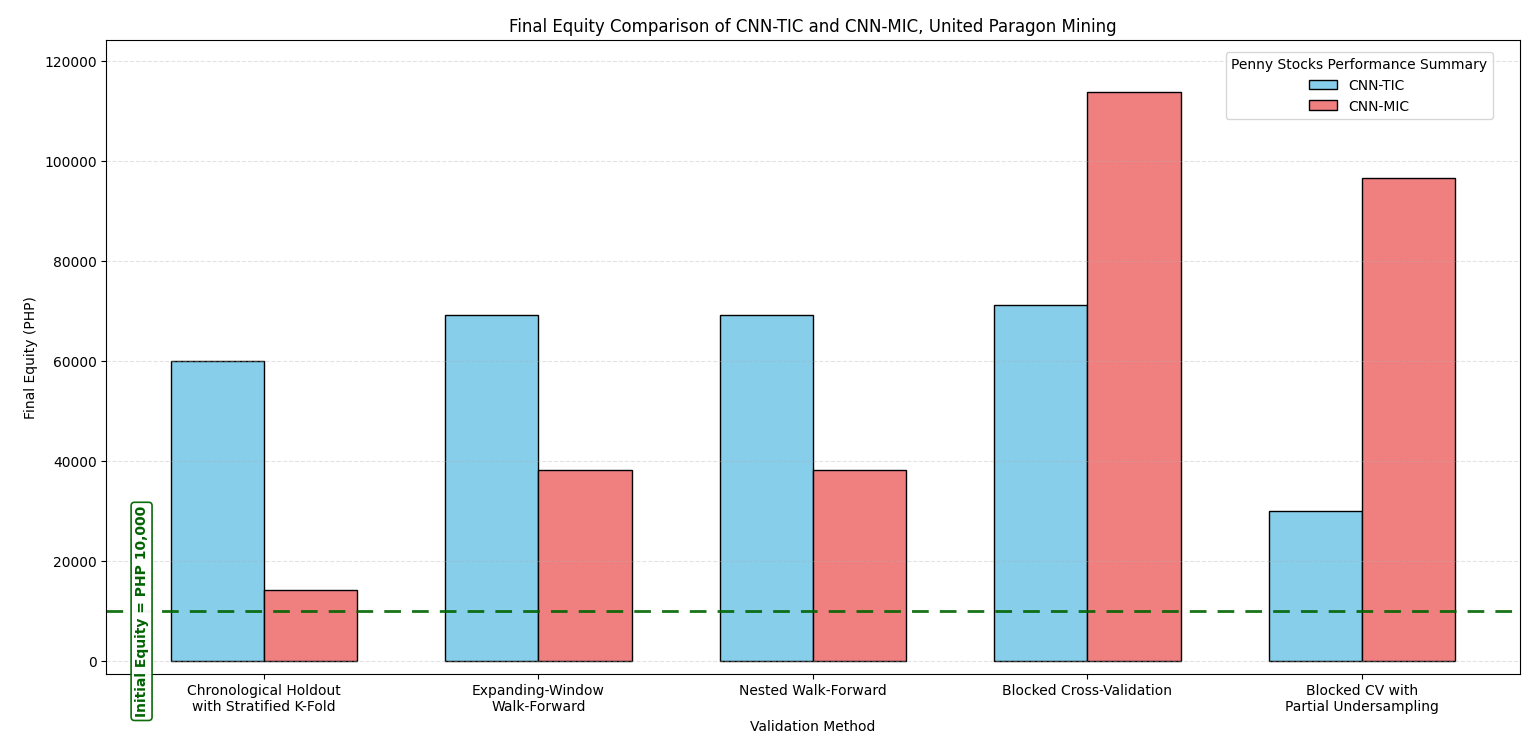
\includegraphics[width=0.8\textwidth]{../figures/UPM_FinancialAccuracy.png}
	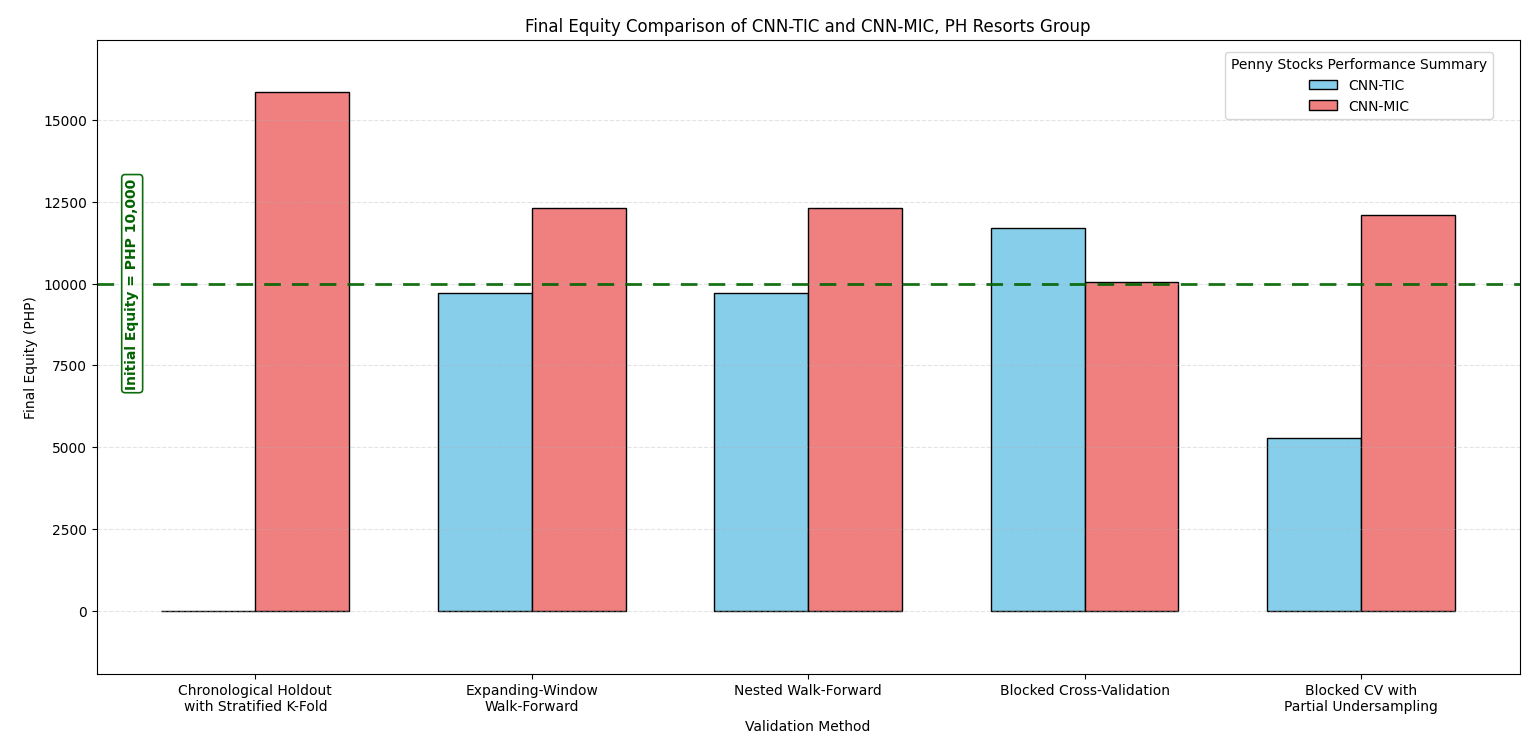
\includegraphics[width=0.8\textwidth]{../figures/PHR_FinancialAccuracy.png}
	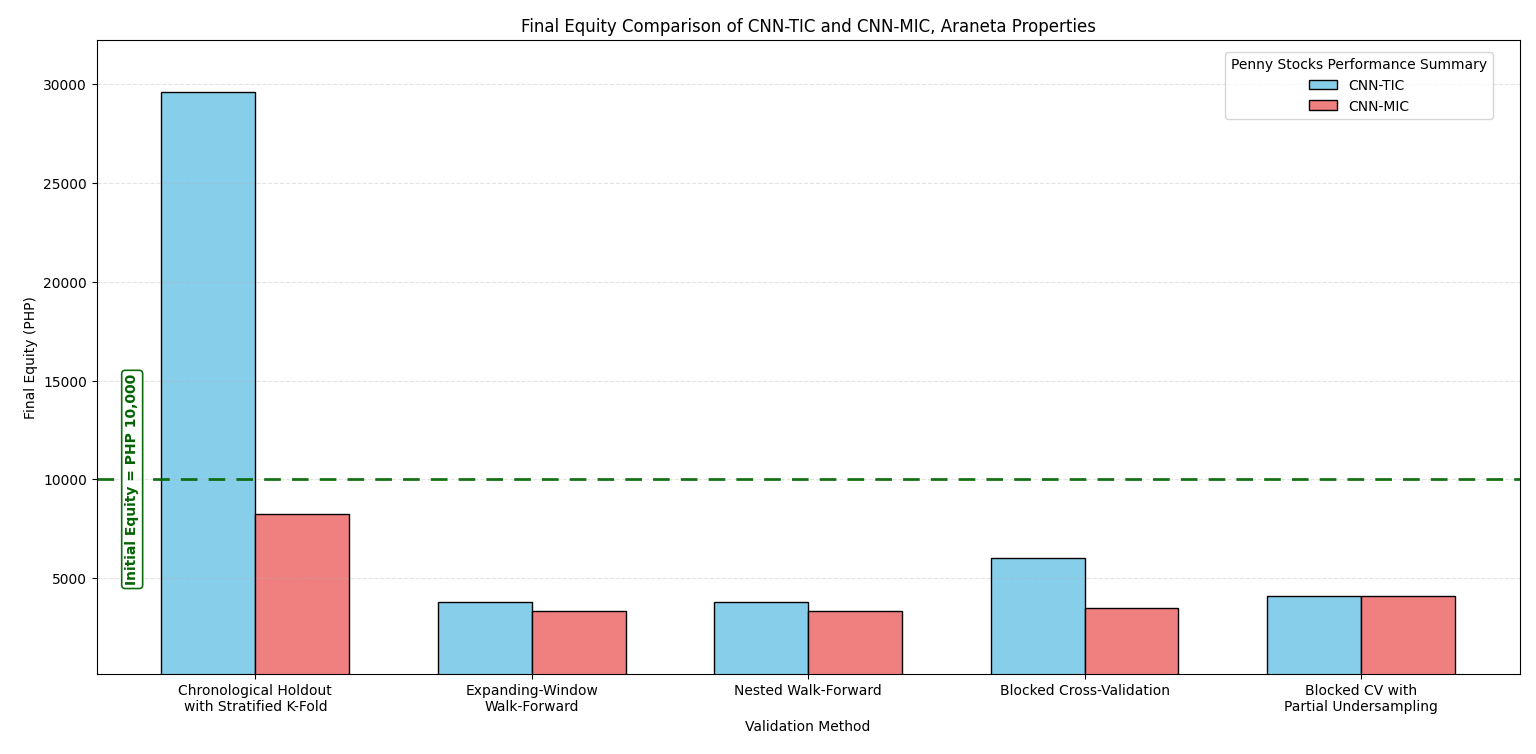
\includegraphics[width=0.8\textwidth]{../figures/ARA_FinancialAccuracy.png}
	
	\captionof{figure}{Final equity performance of CNN--TIC and CNN--MIC across selected penny stocks}
	\label{fig:fin_penny_barplots}
\end{center}

Figures~\ref{fig:test_penny_barplots} and~\ref{fig:fin_penny_barplots} show the test accuracy and final equity performance of CNN--TIC and CNN--MIC across the selected penny stocks. For this group, CNN--TIC generally remained more stable in classification, particularly for PHR and ARA. CNN--MIC showed isolated gains, such as CHV-SKF in UPM and PHR. In financial terms, however, the difference between the two models widened in some cases. CNN--MIC produced markedly higher final equity for UPM under BCV and BCV-PU and also outperformed for PHR in several settings, while CNN--TIC remained stronger for ARA. These results indicate that even when classification gains are limited, macroeconomic integration can still alter trading outcomes substantially in highly volatile equities.

\begin{center}
	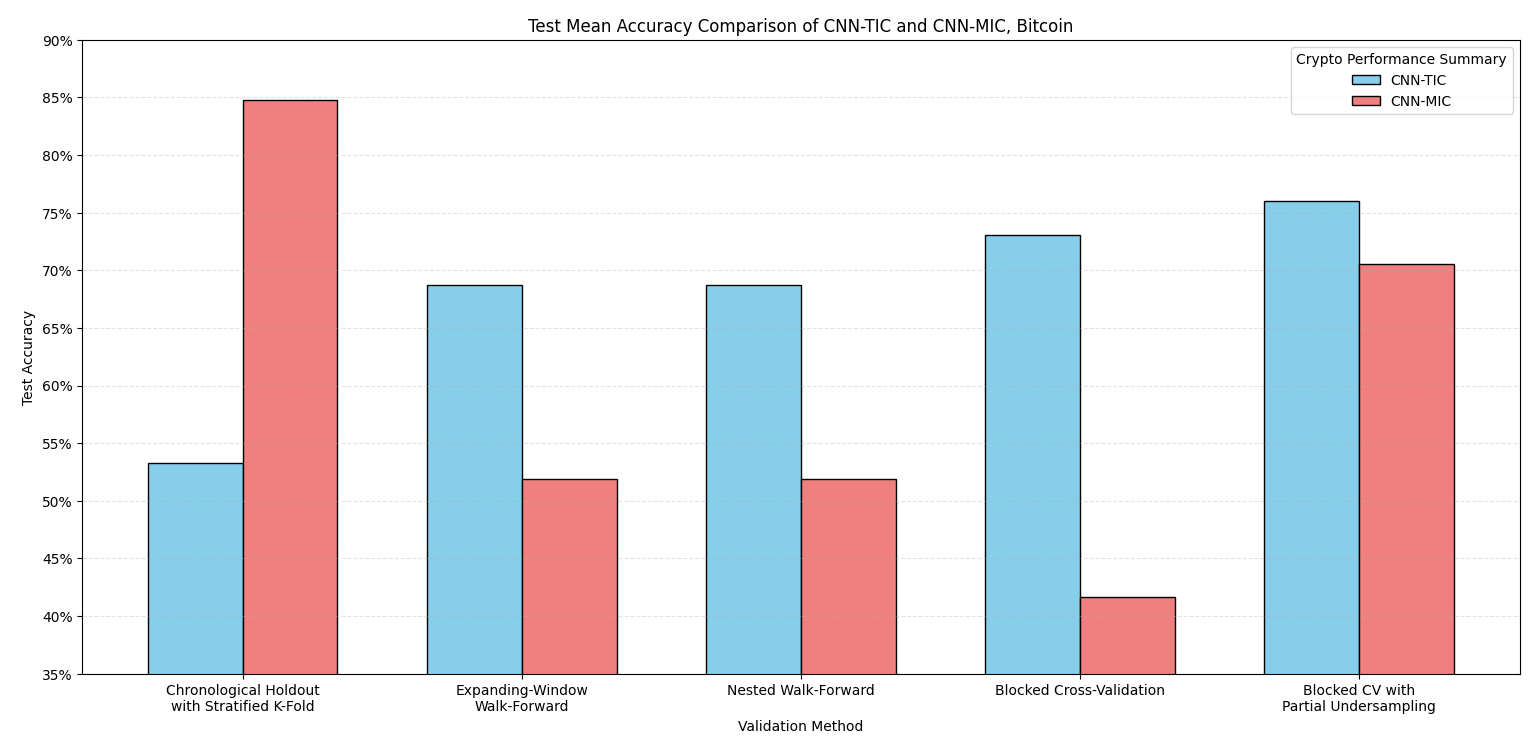
\includegraphics[width=0.8\textwidth]{../figures/BTC_TestAccuracy.png}
	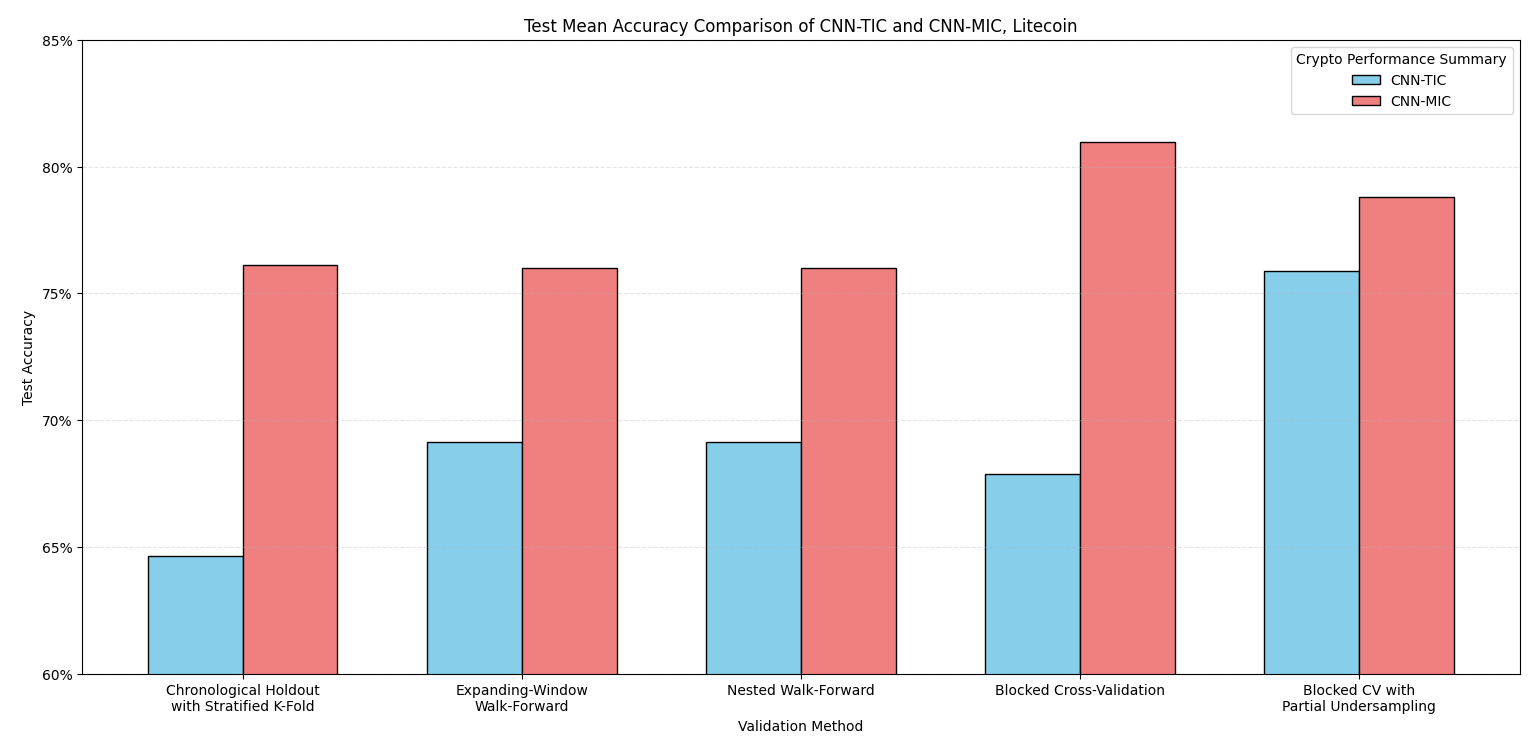
\includegraphics[width=0.8\textwidth]{../figures/LTC_TestAccuracy.png}
	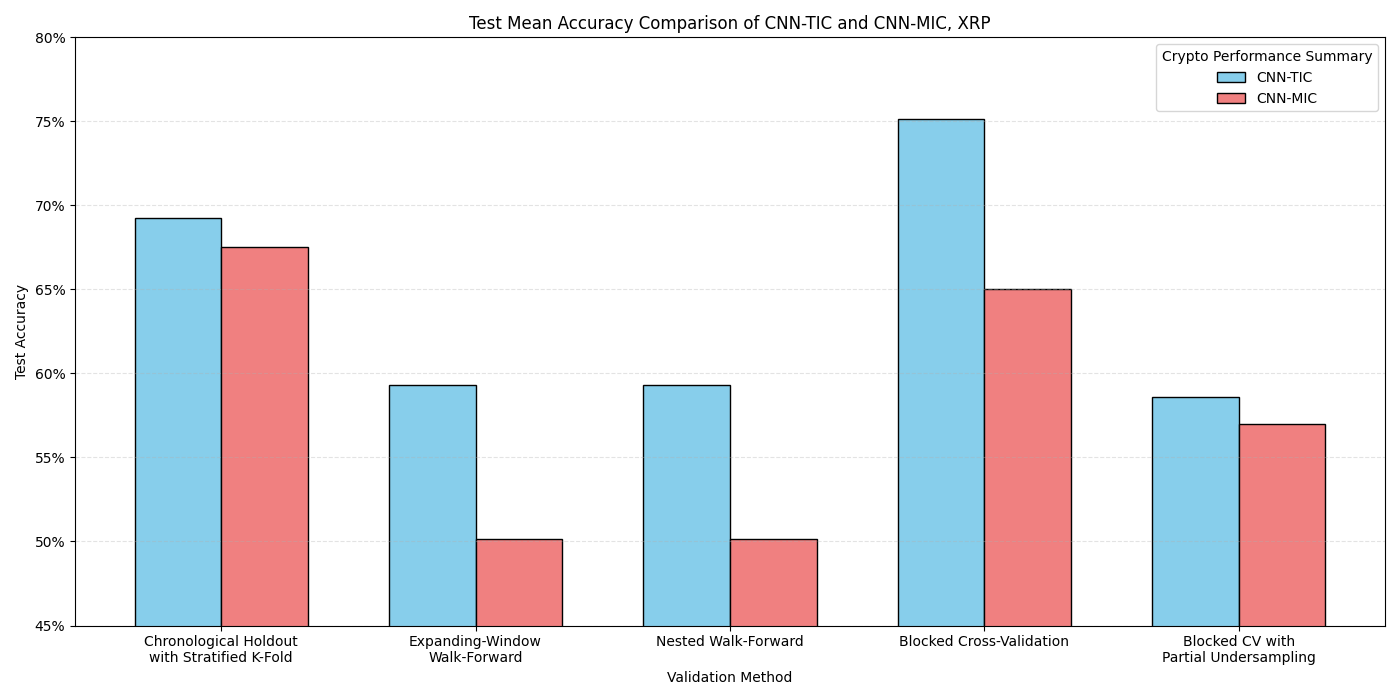
\includegraphics[width=0.8\textwidth]{../figures/XRP_TestAccuracy.png}
	
	\captionof{figure}{Test accuracy performance of CNN--TIC and CNN--MIC across selected cryptocurrency assets}
	\label{fig:test_crypto_barplots}
\end{center}

\begin{center}
	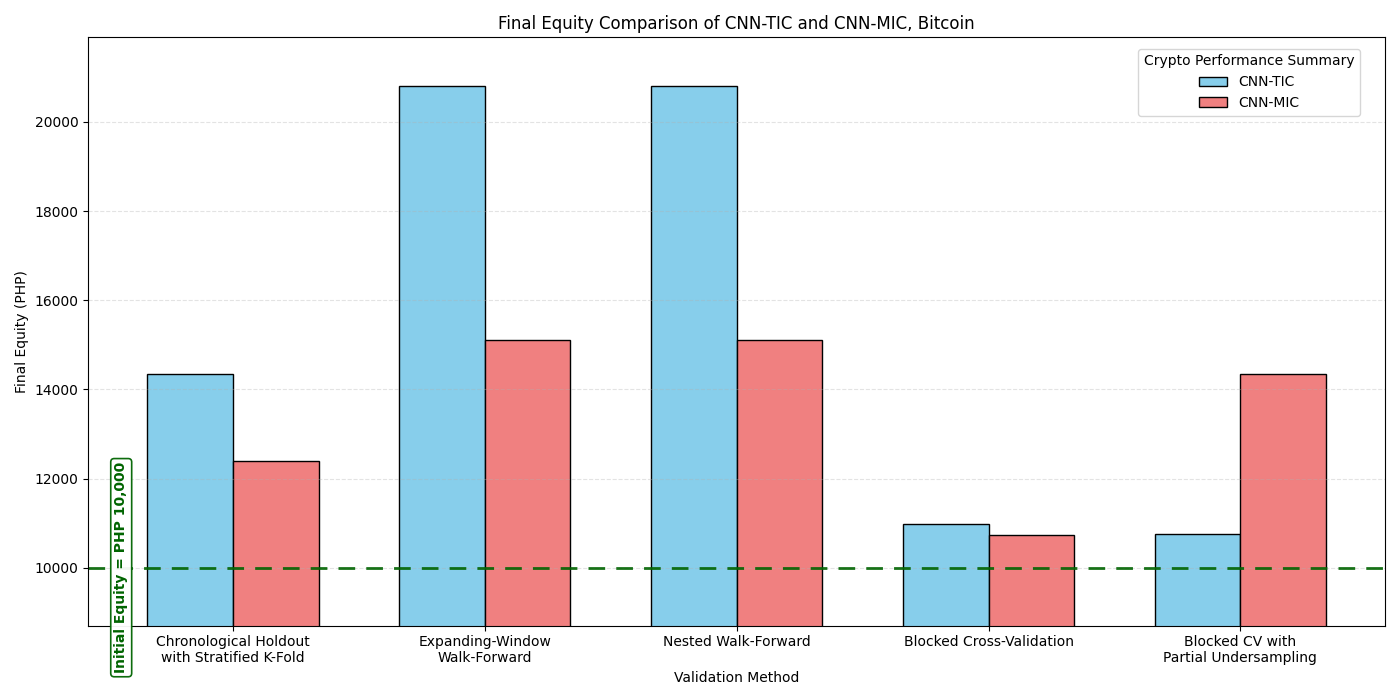
\includegraphics[width=0.8\textwidth]{../figures/BTC_FinancialAccuracy.png}
	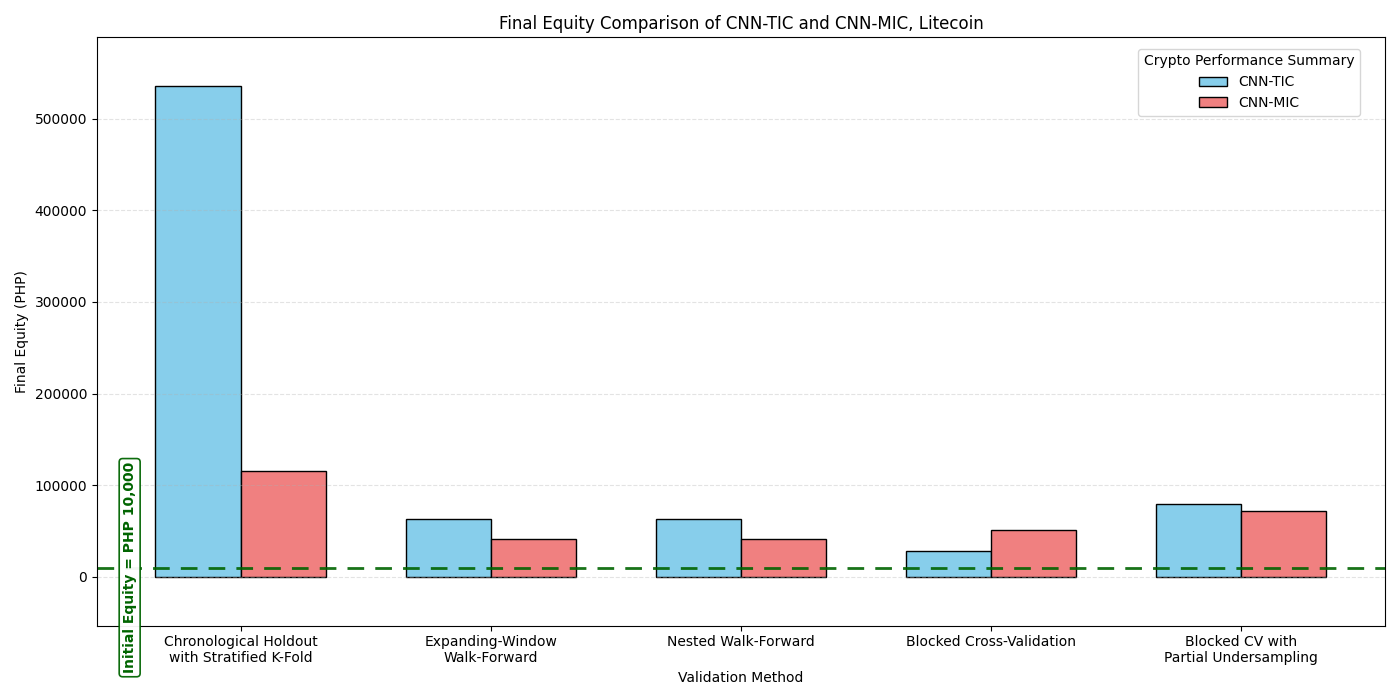
\includegraphics[width=0.8\textwidth]{../figures/LTC_FinancialAccuracy.png}
	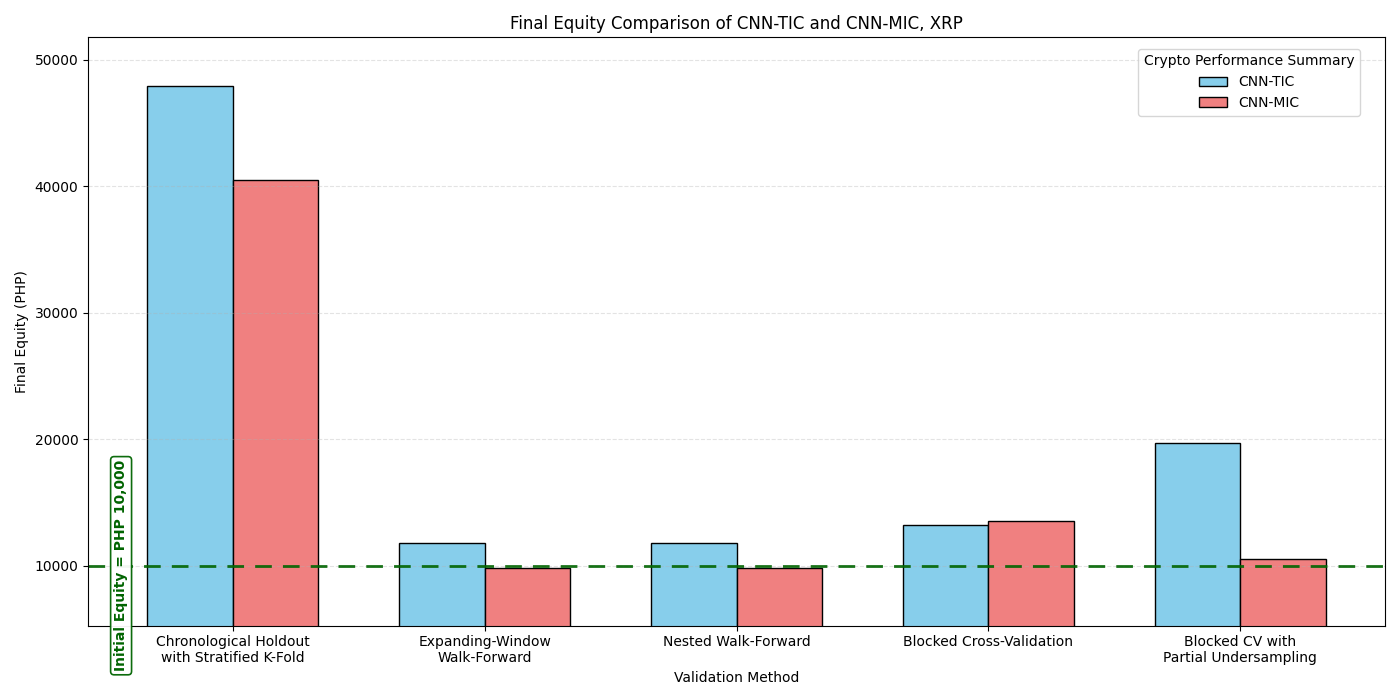
\includegraphics[width=0.8\textwidth]{../figures/XRP_FinancialAccuracy.png}
	
	\captionof{figure}{Final equity performance of CNN--TIC and CNN--MIC across selected cryptocurrency assets}
	\label{fig:fin_crypto_barplots}
\end{center}

Figures~\ref{fig:test_crypto_barplots} and~\ref{fig:fin_crypto_barplots} show the test accuracy and final equity performance of CNN--TIC and CNN--MIC across the selected cryptocurrency assets. For cryptocurrencies, the clearest classification advantage of CNN--MIC appeared in Litecoin, where it outperformed CNN--TIC across all test settings derived from the validation schemes. BTC showed a split pattern, with CNN--MIC performing strongly in CHV-SKF but lagging in several other schemes. XRP remained more favorable to CNN--TIC. The financial results were more conservative. Despite CNN--MIC's classification gains in Litecoin, CNN--TIC still achieved higher final equity in all five configurations. It also remained stronger in most BTC and XRP settings. This result shows that higher classification accuracy does not always translate directly into stronger financial performance. 
In Litecoin, CNN--MIC achieved stronger classification accuracy across the validation-derived test settings, but CNN--TIC still produced higher final equity in all five configurations. 
This means that CNN--TIC may have produced fewer correct predictions overall, but its correct signals were more financially valuable under the trading rules used in this study. 
The result supports the need to evaluate trading models using both predictive and economic metrics, since classification accuracy alone does not capture transaction timing, return magnitude, and portfolio-level outcome \cite{moosa2015directional,fischer2021feature,ozbayoglu2020deep}.

\paragraph{True-label trading performance.}

To further contextualize the financial results of CNN--TIC and CNN--MIC, the true labels were also evaluated as direct trading actions. In this evaluation, the saved Buy, Hold, and Sell labels of each asset were used as the input trading signals. The same financial evaluation procedure was applied, including the initial balance, commission, take-profit, stop-loss, yearly return computation, and final equity calculation used for the CNN-based models.

This evaluation shows the financial performance that can be obtained when the generated labels are used directly as trading signals. The results provide a reference point for comparing the financial outcomes of CNN--TIC and CNN--MIC, since both models attempt to predict the same Buy, Hold, and Sell actions.

The table below presents the financial performance obtained when the true labels were used as trading signals. Among the blue-chip stocks, SMI produced the highest final equity with PHP~71,287.24, while AC and JFC reached PHP~48,134.44 and PHP~39,998.07, respectively. The cryptocurrency assets produced the largest final equities, with LTC reaching PHP~423,881.11, XRP reaching PHP~315,861.28, and BTC reaching PHP~296,652.86. Among the penny stocks, UPM obtained the highest final equity at PHP~77,362.25, followed by ARA and PHR.

\begin{table}[H]
	\centering
	\caption{Financial performance using true labels as trading actions}
	\resizebox{\textwidth}{!}{
		\begin{tabular}{llrrr}
			\toprule
			Asset & Category & Final Equity & Mean Annual Return & Std. Annual Return \\
			\midrule
			AC  & Blue-chip Stocks & 48,134.44  & 121.03\% & 37.96\% \\
			JFC & Blue-chip Stocks & 39,998.07  & 102.31\% & 39.87\% \\
			SMI & Blue-chip Stocks & 71,287.24  & 172.90\% & 79.23\% \\
			ARA & Penny Stocks     & 68,571.52  & 168.64\% & 80.65\% \\
			PHR & Penny Stocks     & 67,070.60  & 163.55\% & 69.10\% \\
			UPM & Penny Stocks     & 77,362.25  & 179.34\% & 36.53\% \\
			BTC & Cryptocurrency   & 296,652.86 & 450.30\% & 110.72\% \\
			LTC & Cryptocurrency   & 423,881.11 & 541.45\% & 21.41\% \\
			XRP & Cryptocurrency   & 315,861.28 & 464.15\% & 140.53\% \\
			\bottomrule
		\end{tabular}
	}
\end{table}

The true-label results are substantially higher than the CNN--TIC and CNN--MIC financial results reported in Appendix~\ref{app:experiment2_tables}. This gap is expected because the true labels are generated from the actual turning points of the price series, while CNN--TIC and CNN--MIC only estimate those labels from technical and macroeconomic image representations. The comparison therefore shows that the labeling method itself can produce strong financial outcomes when used directly, but the CNN models still lose performance when approximating those actions from input features. This supports the need to evaluate the models not only by classification accuracy, but also by how closely their predicted trading actions approach the financial behavior of the true-label reference.

\paragraph{Volatile-period evaluation from 2021 to 2022.}

To further examine the relationship between classification accuracy and profitability, an additional volatile-period evaluation was conducted using 2021 to 2022 as the evaluation window. This period was selected to represent a more unstable market condition following the pandemic-driven disruption in financial markets. The evaluation followed the Chronological Holdout Validation with Stratified K-Fold (CHV-SKF) setup. In this setup, the models were trained using data up to 2020 and evaluated on the period after 2020. 

The volatile-period evaluation used only the prediction rows dated from 2021-01-01 to 2022-12-31. For PSE assets, the first available trading date was 2021-01-04. For cryptocurrency assets, the first available date was 2021-01-01. Classification accuracy and macro F1 were computed from the saved prediction files. Financial performance was computed using the corresponding backtest outputs under the same take-profit, stop-loss, and commission rules used in Algorithm~2.

Table~\ref{tab:volatile-period-performance} summarizes the model performance during the 2021--2022 volatile period. The results show that higher accuracy did not always correspond to higher final equity. CNN--MIC produced higher accuracy in JFC, SMI, PHR, UPM, BTC, LTC, and XRP. However, the higher-accuracy model was not always the more profitable model. For SMI, UPM, BTC, and LTC, CNN--MIC achieved higher classification accuracy, but CNN--TIC produced higher final equity. For AC, the opposite pattern appeared, where CNN--TIC achieved higher accuracy, but CNN--MIC produced higher final equity.

\begin{table}[H]
	\centering
	\caption{Volatile-period performance of CNN--TIC and CNN--MIC using 2021--2022 as evaluation window}
	\label{tab:volatile-period-performance}
	\resizebox{\textwidth}{!}{
		\begin{tabular}{lrrrrrr}
			\toprule
			Asset & TIC Accuracy & MIC Accuracy & TIC Final Equity & MIC Final Equity \\
			\midrule
			AC  & 71.66\% & 61.54\% & 11,993.69 & 14,818.66 \\
			JFC & 65.59\% & 70.85\% & 9,075.38  & 9,251.30  \\
			SMI & 75.10\% & 75.91\% & 18,992.57 & 16,250.71 \\
			ARA & 73.50\% & 73.04\% & 25,221.47 & 15,491.72 \\
			PHR & 58.30\% & 61.94\% & 6,955.87  & 10,722.70 \\
			UPM & 67.49\% & 72.70\% & 11,968.99 & 8,914.22  \\
			BTC & 69.59\% & 83.01\% & 12,660.80 & 12,403.82 \\
			LTC & 62.33\% & 72.60\% & 59,063.82 & 58,106.17 \\
			XRP & 70.41\% & 74.25\% & 36,131.72 & 36,957.03 \\
			\bottomrule
			\end{tabular}
		}
	\end{table}

These results strengthen the main finding of Experiment~2. During the 2021--2022 volatile period, CNN--MIC had the higher accuracy in seven of the nine assets. However, CNN--MIC had the higher final equity in only four assets. This shows that accuracy and profitability can diverge more clearly during unstable market conditions. A model may correctly classify more days overall, but its profitable signals may occur at weaker entry or exit points. 
Likewise, a model with lower accuracy may still produce higher equity if its correct Buy and Sell signals occur near larger price movements. Thus, the volatile-period evaluation supports the use of both predictive metrics and financial metrics when assessing CNN-based trading models.

\subsection{Experiment 3: SHAP-Based Interpretation of CNN--MIC Across Validation Schemes}

 The analysis was applied to the predicted-class outputs of the model and was restricted to correctly predicted test samples in order to focus on feature contributions associated with valid model decisions. This experiment was intended to complement the numerical findings of Experiments 1 and 2 by showing how the model combined technical and macroeconomic information under different evaluation settings.

Across the analyzed SHAP results, technical indicators generally remained the dominant source of information in CNN--MIC. However, macroeconomic variables still showed visible contributions, and their relative importance varied depending on the validation scheme. This indicates that the inclusion of macroeconomic indicators did not replace the technical representation of the model. Instead, it enriched the input space by providing additional context that became more or less useful depending on the evaluation setting.

Figure~\ref{fig:shap_ac_bcvpu_rows} shows the predicted-class SHAP row importance for Ayala Corporation under BCV-PU, which is used here as a representative example. In this scheme, Williams \%R appeared as the most influential technical contributor, followed by CMO and CCI. Among the macroeconomic variables, Reverse Repurchase Rate (RRP) and Purchasing Power of Peso (PPP) showed the strongest contributions, while Oil, Gold, and Inflation Rate had smaller but still visible influence. The figure shows that although macroeconomic variables were meaningfully involved in the prediction process, the dominant contributions still came from technical rows.

\begin{figure}[H]
	\centering
	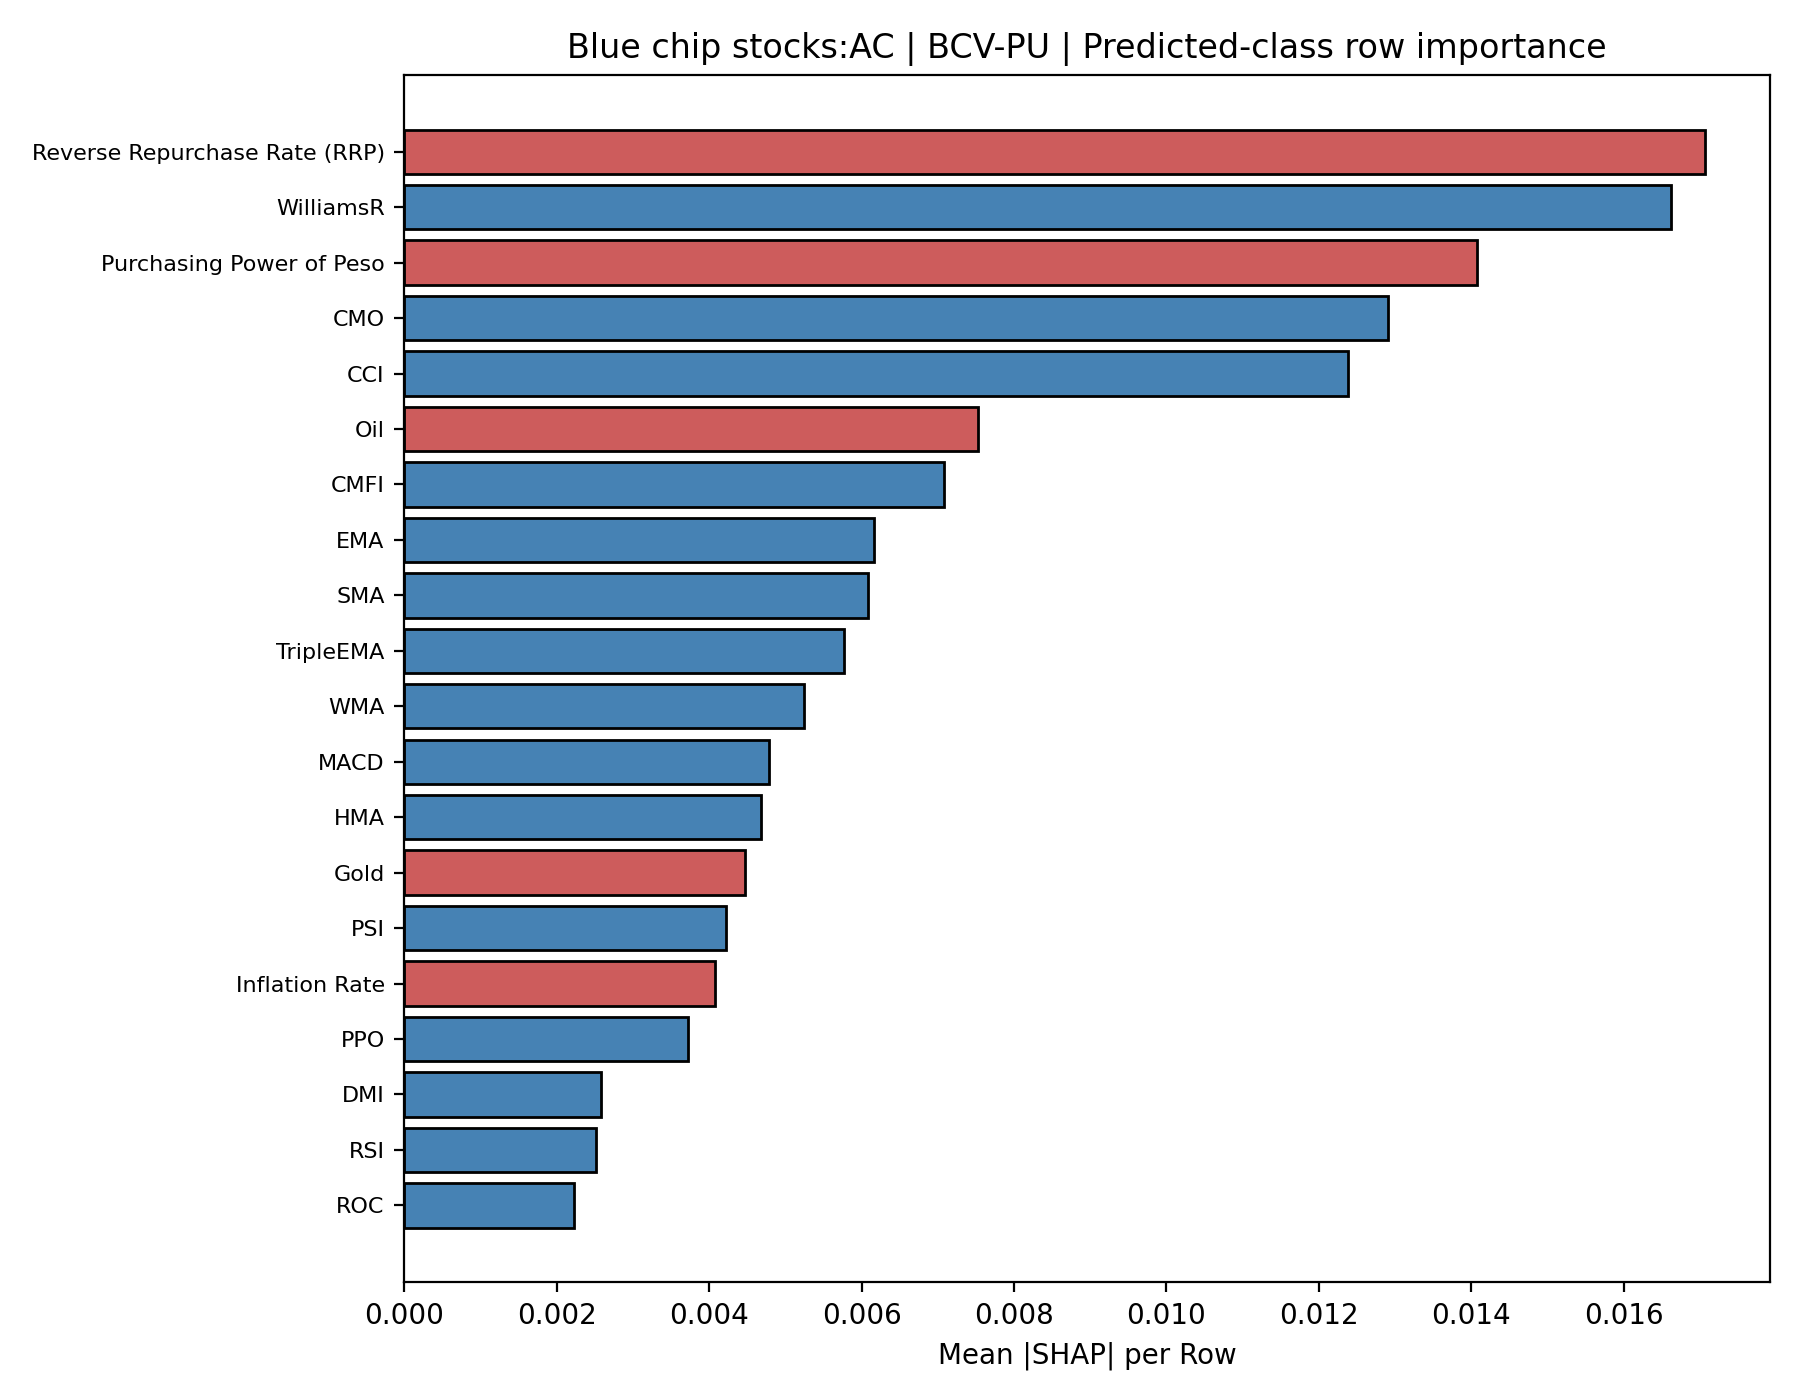
\includegraphics[width=1\textwidth]{../figures/AC_PredictedClassRowImportance.png}
	\caption{Predicted-class SHAP row importance for Ayala Corporation under BCV-PU. }
	\label{fig:shap_ac_bcvpu_rows}
\end{figure}

The remaining validation schemes followed the same general pattern, where technical indicators accounted for the larger share of feature contribution and macroeconomic variables acted as supplementary inputs. What changed across schemes was not the overall dominance of technical information, but the relative strength of the macroeconomic variables and the ranking of the most influential rows. This suggests that the contribution of macroeconomic information in CNN--MIC is sensitive to the structure of the evaluation procedure. In the case of AC, these variables functioned as supporting contextual signals rather than as the primary basis of prediction, which reinforces the broader result of this chapter that macroeconomic integration is condition-dependent and works best as a complement to technical information rather than as a replacement for it. The predicted-class SHAP row importance plots for the remaining assets are presented in Appendix~\ref{app:experiment3_shap}.



